\documentclass[12pt]{article}
\usepackage{amsmath, amsfonts, amsthm, amssymb, math, ifthen, ode}
%\addtolength{\topmargin}{-1in}
%\addtolength{\oddsidemargin}{-0.5in}
%\addtolength{\evensidemargin}{-0.5in}
%\addtolength{\textwidth}{1in}
%\addtolength{\textheight}{1in}


\newcounter{showsolutions}
\setcounter{showsolutions}{1}

\pagestyle{empty}

\title{Math 201: Differential Equations for Engineers\\Lab Manual}
\author{Malcolm Roberts and Samantha Marion}

\begin{document}

\maketitle
%TODO: make title page

Differential equations (abbreviated DEs) are equations involving functions and 
their derivatives. For example, 
\be \label{eg1}
\dd{y}{x} =y
\ee
is a differential equation. In this case, $y$ is a function of the independent 
variable $x$, and we would like to determine $y$. The solution to this
equation is
\be
y = Ce^x,
\ee
with $C$ an arbitrary constant, since $y'=\dd{}{x}Ce^x=Ce^x=y$. That is, if we 
plug $y=Ce^x$ into equation (\ref{eg1}), both sides match. If we modify this
a little bit, say letting $y=Ce^x +x$, then the left hand side doesn't
match the right:
\be
\dd{y}{x} = \dd{}{x}(Ce^x +x) = Ce^x + 1 = y +1 \neq y,
\ee
so it isn't a solution to equation (\ref{eg1}).

An initial value problem (abbreviated as IVP) is a differential equation 
combined with one or more initial conditions. For example
\be
\dd{y}{x}=y, \qquad y(0)=1.
\ee
The differential equation is solved by $y=Ce^x$, for any value of $C$. However,
the only way to satisfy $y(0)=Ce^0=1$ is to set $C=1$. That is, the solution
to the initial value problem is $y=e^x$, since it satisfies both the 
differential equation and the initial conditions.

Differential equations are extremely useful for modelling complex behaviour in 
most sciences. Unfortunately, we do not know how to solve most
differential equations analytically, and in practice we often have to 
make approximations when dealing with real systems. However, when we can solve
DEs analytically, we should, and understanding how to solve simple DEs will
help to understand the properties of solutions of more complicated problems.

\newpage

\section{Lab 1: Separable, linear, and exact equations}

FIXME: separate this into two labs

\subsection{Separable equations}

Separable equations are of the form
\be \label{separable}
  h(y) \dd{y}{x} = g(x).
\ee
These are simple to solve: from equation (\ref{separable}), we can just split
the derivative and integrate: $ h(y)\, dy = g(x) \, dx$ becomes
\be 
  \int h(y) \, dy = \int g(x) \, dx,
\ee
and then all we need to do is find the integral and solve for $y$.\\

\noindent\emph{Example}: Consider the equation
\be \label{separableexample}
  y \dd{y}{x} = \sin(x)
\ee
with initial condition $ y(0) = 1$. Separating and integrating yields
\be 
  \int y \, dy = \int \sin(x) \, dx
  \qquad \implies \qquad 
  \frac{y^2}{2} = -\cos(x) + C
\ee
where $C$ is a constant that will be determined by the initial conditions.
Let us now solve for $y$.
\be 
  y(x) = \pm \sqrt{2 C -2 \cos(x)}.
\ee
Notice that we have two different solutions! We can use the initial condition
$y(0)=1$ to eliminate one. Since 
\be 
  y(0) = \pm  \sqrt{2 C - 2 \cos(0) } = \pm \sqrt{2C-2} =1,
\ee
and $1$ is positive, we must choose the positive root.
Thus, 
\be  
\(C-1\)^2 =1/2
\quad \implies \quad
C=3/2
\quad \implies \quad
y(x) = \sqrt{3 - 2\cos(x)}.
\ee

It's a good idea to check that the solution that you got is correct. This is
pretty easy; just plug the solution into the original equation. From
the above example, $y(x) = 2 \sqrt{\frac{3}{2} - \cos(x)}$, so
\be  
  \dd{y}{x} = \frac{\sin(x)}{\sqrt{3 -2 \cos(x)}}.
\ee
Putting this into equation (\ref{separableexample}) yields
\be 
  y \dd{y}{x}=
  \(\sqrt{3 - 2\cos(x)}\) \times \(\frac{\sin(x)}{\sqrt{3 -2 \cos(x)}}\)
  = \sin(x)
\ee
so we can be sure that we got the correct answer.

\subsection{Linear Equations}

Linear equations have the form
\be \label{linear}
  \dd{y}{x} + P(x) y = Q(x).
\ee
To solve these equations, we use an \emph{integrating factor}. That is, if
we define the integrating factor $\mu$ as
\be 
  \mu(x) \doteq \exp\[ \int P(x) d x \],
\ee
then notice that
\be 
  \dd{}{x}\(\mu y \) = \dd{\mu}{x} y + \mu \dd{y}{x} 
  = \mu P(x) y + \mu \dd{y}{x}.
\ee
So if we multiply equation (\ref{linear}) by $\mu$, we get
\be 
  \dd{}{x}\(\mu y \) = \mu Q,
\ee
which we can now solve by taking the integral of both sides with respect to 
$x$.
FIXME: give the general formula, use it in examples.
\\

\noindent \emph{Example}:
\label{linearsec}
Consider the equation
\be 
  \dd{y}{x} + \frac{y}{x} = 2 e^x.
\ee
We identify $P(x)=1/x$ and $Q(x)=2e^x$. The integrating factor is
\be 
  \mu(x) = \mbox{exp}\[\int \frac{1}{x} \, dx \] = e^{\ln x} = x.
\ee
Then,
\be \label{linearex}
  \dd{}{x} \(x y \) = 2 x e^x
  \quad \implies \quad
  x y = \int 2 x e^x \, dx. 
\ee
To solve this, we use integration by parts. That is, 
$\int u \, dv = uv - \int v\,  du$. We choose $u=x$ and $dv = e^x \, dx$, so
$du = dx$, and $v=e^x$. Thus,
\be 
  \int x e^x \,dx = x e^x + \int e^x \,dx = x e^x + e^x.
\ee
Solving equation (\ref{linearex}) for $y$ yields
\be 
  y = 2 e^x \(1 + \frac{1}{x}\) + \frac{C}{x}.
\ee
We can now use the initial conditions to determine the value of $C$.

% TODO: show how they can check this?

\subsection{Exact Equations}

\begin{definition}\emph{Exact equations.}
Homogeneous first-order differential equations can be written in the form
$M(x,y) dx + N(x,y)dy=0.$ If 
\be 
  \pp{M(x,y)}{y} =   \pp{N(x,y)}{x}
\ee
then the equation is called \emph{exact}.
\end{definition}
The nice thing with exact differentials is that Poincare's lemma implies 
the existence of a function $F$ such that $dF = M(x,y)dx + N(x,y)dy$, and
$dF$, called the differential of $F$, can be thought of as ``how much $F$
changes''. Since $dF=0$, $F$ does not change, i.e.\ it's constant.
Solutions to the exact differential equation are given
implicitly by $F(x,y)=\text{constant}$.

Exact equations are straightforward to solve: after a little bit of trickery, 
we simply integrate. Let 
\be \label{exactsol}
  F(x,y) = \int M(x,y) dx + g(y). 
\ee 
We require that $\pp{}{y}F(x,y)= N(x,y)$, which will allow us to determine 
$g(y)$. That is,
\be 
  \pp{F(x,y)}{y} 
  &=& \pp{}{y}\(\int M(x,y) dx + g(y)\)
  \\
  &=& \int \pp{M(x,y)}{y} dx + \pp{g(y)}{y}
  \\
  &=& N(x,y) + g'(y).
\ee
This tells us what $g'(y)$ is, so we now know $g(y)$ up to some constant
$C$. We can put this into equation (\ref{exactsol}), which gives us the
implicit solution
\be \label{exactimpl}
  F(x,y) =C. 
\ee
In many cases, we can solve for $y$, thus getting an explicit solution 
$y=f(x)$ so that $F(x,f(x))=C$, but sometimes all we have for a solution
is something in the form of equation (\ref{exactimpl}).\\

\noindent\emph{Example}: Solve 
\be 
  y\, dx + \(y^2 + x \) dy =0
\ee
Using the notation above, we have $M(x,y)=y$, and $N(x,y)=y^2 +x$.
This equation is exact, since 
\be  
  \dd{}{y}y = 1 = \dd{\(y^2 +x\)}{x}.
\ee
So write
\be 
  F(x,y) 
  = \int y dx + g(y)
  = xy + g(y).
\ee
We now need to set $\pp{}{y} F = N$, so
\be 
  \pp{}{y}\[xy + g(y)\] = y^2 +x 
\ee
which implies that $g'(y) = y^2$. We integrate this to get 
\be \label{exactC1}
  g(y) = \frac{y^3}{3} + C. 
\ee
The solution is then given by
\be \label{exactC2}
  F(x,y) = xy + \frac{y^3}{3} =C.
\ee
(Note that in the above equation we have played fast and loose with the
undetermined constant $C$; in fact, $C$ changed sign between equation
(\ref{exactC1}) and equation (\ref{exactC2}). We perform this abuse of notation
because $C$ is \emph{undetermined}, so there's not much point nailing it
down to a value until the very last moment.)

\subsection{Equations that can be solved via substitution}

Sometimes it is possible to make a substitution to transform a differential 
equation into something that we already know how to solve. This can be a very 
powerful technique. Unfortunately, each type of equation needs its own 
particular substitution and this makes substitution not as straight forward as 
other techniques.

\subsubsection{Homogeneous Equations}
\be 
\dd{y}{x} = f\(\frac{y}{x}\).
\ee
We solve this by substituting $v=y/x$, so that
\be 
\dd{y}{x} = v + x \dd{v}{x},
\quad \implies \quad
v + x \dd{v}{x} = f(v),
\ee
which is separable.\\

\noindent \emph{Example}:
\be 
\dd{y}{x} = \frac{x}{y}, \mbox{ with } y(1) = 2.
\ee
This is homogeneous, so let $v=y/x$, and then $f(v) = \frac{1}{v}$, so
\be 
v + x \dd{v}{x} = \frac{1}{v} 
\quad \implies \quad
\frac{1}{\frac{1}{v} -v} dv = \frac{1}{x}dx.
\ee
Integrating both sides gives
\be 
\int \frac{v}{1-v^2}dv = \int \frac{1}{x} dx
\quad \implies \quad
-\frac{1}{2} \int \frac{1}{u}du = \ln x+ \ln C
\ee
where we have used the substitution $u = 1-v^2$. Thus,
\be 
\ln\(1-v^2 \) = \ln \frac{C}{x^2}
\ee
which implies that 
\be 
v = \pm \sqrt{1 - \frac{C}{x^2}} 
\quad \implies \quad 
y = \pm x \sqrt{1 - \frac{C}{x^2}}.
\ee
The initial condition is $y(1)=2$, so we choose the positive root, and
find $C$ by setting $x=1$, $y=2$, i.e.\
\be 
2 = 1 \times \sqrt{1-C} 
\quad \implies \quad 
C=-3
\quad \implies \quad 
y = x \sqrt{1 + \frac{3}{x^2}}.
\ee

This would be a good one to check. Note that 
\be 
\dd{y}{x} = \sqrt{1+\frac{3}{x^2}} - \frac{3/x^2}{\sqrt{1+\frac{3}{x^2}}}
= \frac{1}{\sqrt{1+\frac{3}{x^2}}}
= \frac{x}{y},
\ee
so the solution is correct.

\subsubsection{Bernoulli Equations}
Bernoulli equations are differential equations of the form
\be 
\dd{y}{x} + P(x) y = Q(x)y^n
\ee
where $n$ can be an integer or a rational number. Note that if
$n=0$ or $n=1$, then this is just a linear equation.

We solve this by substituting $v=y^{1-n}$, so that
\be 
\dd{v}{x} = \(1-n\)y^{-n}\dd{y}{x}
\quad \implies \quad
\frac{1}{1-n} \dd{v}{x} + P(x)v = Q(x),
\ee
which is a linear equation.\\

\noindent\emph{Example}:
\be 
\dd{y}{x} -\half \frac{y}{x} = -e^x y^3
\ee
Since $n=3$, choose $v=y^{-2}$. Then
\be 
\dd{v}{x} = -2 y^{-3} \dd{y}{x} 
\quad \implies \quad
\dd{v}{x} = -2 y^{-3}\( \half \frac{y}{x}  - e^x y^3\)
\quad \implies \quad
\dd{v}{x} + \frac{v}{x} = 2 e^x,
\ee
which is a linear equation given as the example from section \ref{linearsec}.


%\subsubsection{Equations with Linear Coefficients}
% Question: doesn't case 1 follow from case 2?
% Sam's answer: Yes, I believe it does
%\be
%\(a_1 x + b_1 y + c_1\)dx +2 \(a_2 x + b_2 y + c_2\)dy =0
%\ee
%We deal with equations where $a_1 b_2 \neq a_2 b_1$, for which there
%are two cases:
%\begin{enumerate}
%\item if $c_1=c_2=0$, then
%\be
%\dd{y}{x} = -\frac{a_1 + b_1 \(y/x\)}{a_2+ b_2 \(y/x\)},
%\ee
%which is homogeneous.
%\item if either $c_1$ or $c_2$ is not zero, then we use the substitution
%$x=u+h$ and $y=v+k$, with $h$ and $k$ constants which obey the relationship
%\be
%a_1h + b_1 k + c_1 &=&0 \\ \nonumber
%a_2h + b_2 k + c_2 &=&0 .
%\ee
%This reduces the problem to 
%\be
%\dd{v}{u} = -\frac{a_1 + b_1 \(v/u\)}{a_2 + b_2 \(v/u\)},
%\ee
%which is homogeneous in $u$ and $v$.
%\end{enumerate}

\subsection{Problems}

\begin{enumerate}

\item
% a linear equation
Solve the initial value problem
\bee
&&\qquad(x^2 + 1) \frac{dy}{dx} + 4xy = 4x \\ \nonumber
&&y(0) =\ 0\ \text{ or }\ 1\ \mbox{ (choose one, and circle your choice)}
\eee

\item
% an exact equation
Solve the equation
\bee
(2xy + 3) dx + (x^2 - 1) dy = 0
\eee

\item
 Joe headed out to the bar in his new Thinsulate jacket, but drank 
too much and passed out on the way home. Ignoring the heat that his body
produces, his temperature is determined by Newton's law of cooling.
Determine Joe's temperature $T$ at time $t$ by solving Newton's law of cooling,
both as a separation problem and a linear problem
\bee
\dd{T}{t} = -r\(T - T_\text{env}\),
\quad
T(0)=37,\, T_\text{env}=-40,\, r=5 \, \(\text{Thinsulate's r-value}\)
\eee
% todo: write solutions
% TODO: does this work with C rather than K?

\item 
Solve the logistic map,
\bee
\dd{y}{x} = y - y^2.
\eee
as both a separable equation and a Bernoulli equation
% TODO: write solutions

\item
Solve the differential equation
\bee
\dd{y}{x} = \frac{x + y}{x}.
\eee
% NB: this is a homogeneous equation
% FIXME: add initial value?
% TODO: write solutions

\item
Solve the differential equation
\bee
\dd{y}{x} = \frac{y}{x} + x^2y^2.
\eee
% NB: this is a Bernoulli equation

\item
  Equations of the form $\dd{y}{x} = f(ax+by)$ may be transformed into a 
  separable equation via the substitution  $v=ax + by$. Using this technique,
  solve the differential equation
  \bee 
  \dd{y}{x} = - \(4x -y\)^2
  \eee
  \hidesolution{
    Let $v=4x-y$, so $y'=4-v'$. Then
    \bee 
    v' = v^2 +4 = (v-2)(v+2),
    \eee
    which is separable. That is, $\frac{dv}{(v-2)(v+2)} = dx$, so, using
    partial fractions,
    \bee
    \int \frac{1/4}{v-2} -\frac{1/4}{v+2} \, dv
    = \frac{1}{4} \ln\abs{v-2} - \frac{1}{4} \ln\abs{v+2} = x + C.
    \eee
    Substituting $v=4x-y$ back in, we get the implicit solution
    \bee
    \ln\abs{\frac{4x-y-2}{4x-y+2}} = 4x +C.
    \eee
    Solving for $y$ yields
    \bee
    y = \frac{Ce^{4x}\(4x+2\) -4x +2}{1-Ce^{4x}}.
    \eee
  }

\item
  Equations of the form
  \bee
  \(a_1 x + b_1 y + c_1\)dx +2 \(a_2 x + b_2 y + c_2\)dy =0
  \eee
  can be transformed into homogeneous equations by using the substitution
  $x=u+h$ and $y=v+k$, with $h$ and $k$ constants which obey the relationship
  \bee
  a_1h + b_1 k + c_1 &=&0 \\ 
  a_2h + b_2 k + c_2 &=&0 .
  \eee
  This reduces the problem to 
  \bee
  \dd{v}{u} = -\frac{a_1 + b_1 \(v/u\)}{a_2 + b_2 \(v/u\)},
  \eee
  which is homogeneous in $u$ and $v$.
  Solve the differential equation
  \bee
  \(2y + 2\) dx + \(x +y+2\) dy=0
  \eee
  using this technique.

  \item
    Give the general solution to the differential equation
    \be
    \ddt{y} = 1 + \frac{1}{y^2}
    \ee
    \hidesolution{
      This is a separable equation:
      \bee
      \frac{dy}{1+\frac{1}{y^2}} = dt 
      \implies
      \int dt = \int  \frac{dy}{1+\frac{1}{y^2}} 
      \eee
      But, since
      \bee
      \frac{1}{1+\frac{1}{y^2}} = \frac{y^2}{y^2+1} = 1 - \frac{1}{1+y^2}
      \eee
      so
      \bee
      t = \int  \(1 - \frac{1}{1+y^2}\) dy = y + \arctan y + C,
      \eee
      which implicitly defines $y(t)$.
    }

  \item
    Solve the following differential equation:
    \be
    \dd{y}{x} = \frac{y}{x} + x^2 y^2
    \ee
    \hidesolution{
      This is a Bernoulli equation with $n=2$, so set $v=y^{1-n}=y^{-1}$. Then,
      \bee
      \dd{y}{x} = \frac{-1}{x^2}\dd{v}{x}.
      \eee
      Then,
      \bee
      \frac{-1}{v^2}v' - \frac{1}{xv} = \frac{x^2}{v^2}
      \implies
      v' = \frac{v}{x} - x^2
      \eee
      Now, let $w=v/x$, which implies that 
      \bee
      w + x \dd{w}{x} = w -x^2 \implies \dd{w}{x} = -x^2
      \eee
      Thus, $w = - \half x^2 + C$, so
      \bee
      w=\frac{v}{x} = \frac{1}{xy} \implies \frac{1}{y} = \frac{-x^3}{2} + Cx
      \implies y = \frac{1}{-x^3/2 + Cx}.
      \eee
    }

\end{enumerate}



\newpage
\section{Second-order Linear Equations}
% Text chapter 4.2
Let $a,b,c$ be real numbers. Second order equations of the form 
\be \label{sec2hom}
a \ddtwo{y}{t} + b \dd{y}{t} + cy =0
\ee
are linear in $y$. If both $y_1$ and $y_2$ are solutions to 
equation (\ref{sec2hom}), and $\alpha$ and $\beta$ are constants, then
\newcommand\ycomb{\alpha y_1 + \beta y_2}
\be 
&& a \ddtwo{\(\ycomb\)}{t} + b \dd{\(\ycomb\)}{t} + c \(\ycomb \)
\\  \nonumber
&&= \alpha\(a \ddtwo{y_1}{t} + b \dd{y_1}{t} + cy_1 \)
+\beta\(a \ddtwo{y_2}{t} + b \dd{y_2}{t} + cy_2 \)
\\ \nonumber
&&= \alpha \(0\) +\beta \(0\) =0,
\ee
In other words, $\ycomb$, which is a linear combination of $y_1$ and $y_2$, is 
also a solution to equation (\ref{sec2hom}). Being able to use this linearity 
is a powerful tool that we can use to solve this very important type of 
differential equation. We will, in general, have two solutions to these 
second-order differential equations, and we will need two initial values to 
fully determine the solution. This is expressed in the following theorem:

\begin{theorem}
  Let $b$, $c$, $Y_0$, and $Y_1 \in \mathbb{R}$.
  Then, the initial value problem
  \be
  y'' + by' + cy =0, \qquad y(0)=Y_0, \quad y'(0)=Y_1
  \ee
  has a unique solution.
\end{theorem}

\subsection{Homogeneous Linear Equations}
The behaviour of these systems is basically exponential. To see this,
set $y=e^{rt}$. Then, putting this into equation (\ref{sec2hom}), we get
\be 
a r^2 e^{rt} + b r e^{rt} + ce^{rt}
= e^{rt} \( ar^2 + br + c\) =0.
\ee
Since $e^{rt}$ is never zero, there is no harm in dividing by it. This leaves
us with the \emph{characteristic equation},
\be 
ar^2 + br + c =0,
\ee
which allows us to determine $r$ using the quadratic formula. In this way
we get two solutions, $y_1=e^{r_1 t}$ and $y_2=e^{r_2 t}$, from the two
solutions $r_1$ and $r_2$ of the characteristic equation.\\

\noindent\emph{Example}: Solve the second-order homogeneous equation
\be 
\ddtwo{y}{t} - y =0,
\ee
with initial conditions $y(0) =1, \, y'(0) =0.$\\
\noindent\emph{Solution}: 
Setting $y=e^{rt}$, this becomes
\be 
e^{rt} \(r^2 -1 \) = e^{rt} \(r-1\)\(r+1\) =0,
\ee
so $r_1=-1$, and $r_2=1$. Thus,
\be 
y_1(t) = e^{-t}, \qquad y_2(t) =e^t.
\ee
The solution $y$ is therefore a linear combination of $y_1$ and $y_2$. That is,
\be 
y(t) = \alpha y_1(t) + \beta y_2(t) = \alpha e^{-t} + \beta e^t,
\ee
for some constants $\alpha$ and $\beta$ that are determined by the initial
conditions. Since $y(0)=1$,
\be \label{sec2ab1}
y(0) = \alpha +\beta =1.
\ee
Since $y'(0)=0$, and $y'(t) = -\alpha e^{-t} + \beta e^t$,
\be \label{sec2ab2}
y'(0) = -\alpha + \beta =0.
\ee
Combining equations (\ref{sec2ab1}) and (\ref{sec2ab2}), it is easy to see that
$\alpha = \beta =\half$. The solution is therefore
\be 
y = \frac{e^{-t} + e^t}{2}.
\ee

\subsection{Dealing with complex roots}
%Text section 4.3
So far, we've seen only problems where the roots of the characteristic 
equation are real. Of course, this isn't always the case, but we can deal with 
this using \emph{Euler's Formula},
\be 
e^{i\theta} = \cos(\theta) + i \sin(\theta).
\ee
For example, if we get $r_{1,2}= 4\pm 2i$, then solutions are a linear
combination of
\be 
e^{(4+2i)t}=e^{4t}e^{i2t}=e^{4t} \(\cos(2t) + i \sin(2t)\)
\ee
and
\be 
e^{(4-2i)t}=e^{4t}e^{-i2t}=e^{4t} \(\cos(2t) - i \sin(2t)\).
\ee
An easy way to get all linear combinations is to just set
\be 
y_1(t) = e^{4t} \cos(2t), \qquad y_2(t) = e^{4t} \sin(2t).
\ee
\\

\noindent\emph{Example}: Give the general solution to
\be 
\ddtwo{y}{t} + 1 =0
\ee
with initial conditions $y(0) =1, \, y'(0) =0.$\\
\noindent\emph{Solution}:
The characteristic equation is
\be 
r^2 +1 =0 \quad \implies \quad r = \pm i.
\ee
The solution is then a linear combination of
\be 
y_1(t) = e^{0t}\cos(t) = \cos(t), \qquad
y_2(t) = e^{0t}\sin(t) = \sin(t)
\ee
Setting $y(t)=\alpha \cos(t) + \beta \sin(t)$, we can input the initial
conditions to get
\be 
y(0) &=& \alpha\cos(0) + \beta\sin(0) = \alpha =1,
\\
y'(0) &=& -\alpha\sin(0) + \beta\cos(0) =\beta =0.
\ee 
The solution to the IVP is then
\be 
y(t) = \cos(t).
\ee

\subsection{Dealing with repeated roots}
In the above section, we were lucky, since we had two independent roots.
Two independent roots gave two independent solutions $y_1$ and $y_2$, which
we used to solve the two initial values for the problem. When we have 
repeated roots, we still need to make sure that we have two independent 
solutions. How do we get this? Well, just multiply one solution by $t$.

For example, suppose that we solved the characteristic equation and got 
$r_1=r_2=r$. We still get one solution out of this, namely
\be 
y_1(t) =e^{rt}.
\ee
To get the second solution, just take
\be 
y_2(t) = t y_1(t) = t e^{rt}.
\ee
This works since $\ddtwo{t}{t}=0$, so the extra $t$ in $y_2$ is eventually
killed, and everything cancels out nicely.
\\

\noindent\emph{Example}: Give the general solution to
\be 
\ddtwo{y}{t} - 2 \dd{y}{t}+1 =0
\ee
with initial conditions $y(0) =1, \, y'(0) =0.$\\
\noindent\emph{Solution}:
The characteristic equation for this problem is
\be 
r^2 - 2r +1 = (r-1)(r-1) =0,
\ee
which has the double root $r_1=r_2=1$. Thus, set 
$y_1(t) = e^t$ and $y_2=t e^t$, so
\be 
y = \alpha e^t + \beta t e^t
\ee
Now,
\be 
y(0) = \alpha = 1.
\ee
For the second condition, calculate that 
$y'(t) = \alpha e^t + \beta e^t + \beta te^t$. Thus
\be 
y'(0) = \alpha + \beta =0.
\ee
Thus, $\alpha=1$ and $\beta =-1$, so the solution is
\be 
y(t) = e^t - te^t.
\ee


\subsection{Problems}

\begin{enumerate}

\item 
  % Real roots
  Solve the IVP
  \bee 
  2 y'' + 5y' + 2y =0
  \eee
  with initial conditions $y(0)=0$ and $y'(0)=3/2$.

\item 
  Solve the IVP
  % imaginary roots
  \bee
  2 y'' + 8y =0
  \eee
  with initial conditions $y(0)=1$ and $y'(0)=2$.

\item 
  Solve the IVP
  % complex roots
  \bee
  y'' + 2y' + 4y=0
  \eee
  with initial conditions $y(0)=0$ and $y'(0)=2$.
  %r = -1 \pm i \sqrt{3}
  % y =2 \sqrt{3} e^{-t} \sin(\sqrt{3}t\)

\item 
  Prove Euler's formula using differential equations. \\
  Consider the IVP 
  \bee
  y'' +y =0, \qquad y(0)=1, \quad y'(0)=i.
  \eee
  \begin{enumerate}
    \item Step 1: Show that $\{y_1=\cos(t),y_2=\sin(t)\}$ are solutions
      to the differential equation. Find a solution $y=\alpha y_1 + \beta y_2$
      to the IVP.
    \item Step 2: Using the characteristic equation, find a different pair
      of solutions $\{y_1,y_2\}$ made up of complex exponentials. Find a 
      solution $y=\alpha y_1 + \beta y_2$ to the IVP.
    \item Step 3: Use a theorem to show that these two solutions must be 
      identical, thereby proving Euler's formula.
  \end{enumerate}

\item
  % Mazowita's question. Solution is tex'd.
  Find the general solution of the differential equation 
  \bee
  10, \! 000 \, y'' - 100, \! 000 \, y' + 250, \! 000 \, y = 0.
  \eee


\item
  % Mazowita's question. Solution is tex'd.
  Solve the IVP
  \bee
  y'' + 4y' + 5y = 0
  \eee
  with $y(\pi) =\ e^{-\pi},$ $y' (0) = \sqrt{\pi} + 2e^\pi$.

\end{enumerate}

\newpage
\section{Non-homogeneous Second-Order Linear Equations}

\subsection{Method of Undetermined Coefficients}
% Text section  4.4
The next step is to add a function to the right-hand side of equation 
(\ref{sec2hom}), so that we get
\be 
a y'' + b y' + cy =f(t).
\ee
Then what we have is a \emph{non-homogeneous equation} and we say that equation 
$a y'' + b y' + cy =0$ is the corresponding homogeneous equation.

In this section, we are going to restrict ourselves to a couple of choices
for $f(t)$ so that we can use the method of \emph{undetermined coefficients},
also known as \emph{we can probably guess what the answer is, so let's do 
that}.

The idea behind this method is trying to find the particular solution $y_p$,
which has the property
\be \label{yp}
a y_p'' + b y_p' + cy_p =f(t),
\ee
though it need not match the initial conditions. For instance, if 
$f(t)=\sin(t)$, guessing that $y_p = A \sin(t) + B \cos(t)$ would probably do
the trick. We can just substitute $y_p = A \sin(t) + B \cos(t)$ into equation
(\ref{yp}) in order to find the values of $A$ and $B$ that work. 

Here is a table that will guide you, young jedi:
\be 
\begin{tabular}{ l |  l }
  $f(t)$ & $y_p$  \\
  \hline	
  $ke^{at}$ & $Ce^{at}$  \\
  $kt^n$ & $C_n t^n + C_{n-1}t^{n-1} + \dots + C_1 t + C_0 $  \\
  $k \cos(at)$ or $k \sin(at)$ & $K \cos(at) + M\sin(at)$ \\
  $kt^n e^{at}$ & $e^{at}\(C_n t^n + C_{n-1}t^{n-1} + \dots + C_1 t + C_0\)$ \\
  $k t^n \cos(at)$ or $k t^n \sin(at)$ & 
  $\(C_nt^n + \dots +C_0 \)\cos(at) + \(D_nt^n + \dots + D_0 \)\sin(at)$ \\
  $ke^{at} \cos(bt)$ or $ke^{at} \sin(bt)$ & 
  $e^{at}\(K \cos(at) + M\sin(at)\)$ \\
  $k t^n e^{at }\cos(bt)$ or $k t^n e^{at} \sin(bt)$ & 
  $\(C_nt^n + \dots +C_0 \)e^{at}\cos(bt) 
  + \(D_nt^n + \dots + D_0 \)e^{bt}\sin(bt)$ \\
\end{tabular}
\ee
Finally, if your guess ends up being a polynomial times a linear 
combination of the solutions to the corresponding homogeneous equation (known 
as $y_1$ and $y_2$ in previous lab), then multiply your 
guess by $t$ until it isn't. For example, if $y_1=e^t$, $y_2=e^{2t}$, and 
$f(t)=t^2e^t$, then you would choose $y_p = t\(C_2 t^2 + C_1 t + C_0 \)e^t$. 
If $y_1=e^t$, $y_2=t e^t$, and $f(t)=t^2e^t$, then you would choose 
$y_p = t^2 \(C_2 t^2 + C_1 t + C_0 \)e^t$. 

Once you have determined $y_p$, combine it with the homogeneous solutions
to give the general solution
\be
y(t) = \alpha y_1(t) + \beta y_2(t) + y_p(t) 
\ee
to match the initial conditions.
\\

\noindent \emph{Example}: 
Solve the IVP 
\be \label{undetceg}
y'' -3y' +2 y = t
\ee
with $y(0) = 3/4$ and $y'(0) = 3/2$.\\
\noindent \emph{Solution}:
This has characteristic equation
\be
r^2 -3r +2 = (r-1)(r-2) \quad \implies \quad r_1=1, \, r_2=2,
\ee
so the homogeneous solutions are $y_1(t) = e^t, \, y_2=e^{2t}$. Since
$f(t)=t$ is not a linear combination of $y_1$ and $y_2$, we can just choose
$y_p = C_1 t + C_0$. Putting this into equation (\ref{undetceg}), we get
\be
\ddtwo{(C_1 t + C_0)}{t} -3\dd{(C_1 t + C_0)}{t} + 2 \(C_1 t + C_0\) =t
\quad \implies \quad
-3 C_1 + 2C_1 t + 2C_0 = t,
\ee
so $C_1=1/2$ and $C_0=3/4$. Thus, $y_p = \frac{t}{2} +\frac{3}{4}$, and the 
general solution is
\be
y = \alpha e^t + \beta e^{2t} + \frac{t}{2} +\frac{3}{4}.
\ee
Now, we satisfy the initial conditions: 
\be
y(0) = \alpha + \beta +\frac{3}{4} = \frac{3}{4} 
\quad \implies \quad \alpha+\beta=0,
\ee
and
\be
y'(0) = \alpha + 2\beta + \half = \frac{3}{2} 
\quad \implies \quad \alpha+2 \beta=1 
\ee
so $\alpha=-1$ and $\beta =1$. The solution is therefore
\be
y(t) = -e^t +e^{2t}  + \frac{t}{2} +\frac{3}{4}.
\ee

Let's check this solution. We have
\be
y(t) &=& -e^t +e^{2t}  + \frac{t}{2} +\frac{3}{4}
\\
y'(t) &=& -e^t +2e^{2t}  + \frac{1}{2}
\\
y''(t) &=& -e^t +4 e^{2t}
\ee
Putting these into equation (\ref{undetceg}) yields
\be
&&y'' - 3 y' + 2 y
\\ 
&&= \(-e^t + 4 e^{2t}\) 
-3 \(-e^t +2e^{2t}  + \frac{1}{2} \)
+2 \(-e^t +e^{2t}  + \frac{t}{2} + \frac{3}{4} \) = t,
\ee
as required.

\subsection{Superposition Principle}
Suppose that we know the solution $y_{1,p}$ to
\be
  ay'' + by' + cy = f(t)
\ee
and the solution $y_{2,p}$ to
\be
  ay'' + by' + cy = g(t).
\ee
We can use these to determine the solution to the more difficult problem
\be \label{super}
  ay'' + by' +cy = A f(t) + B g(t)
\ee 
by using the fact that the differential operator 
\be
L = a \ddtwo{}{t}  + b \dd{}{t} + c
\ee
is linear. That is, for constants $\alpha$ and $\beta$
\be
  L\(\alpha y_{1,p} + \beta y_{2,p} \)
  &=&
  a \(\alpha y_{1,p} + \beta y_{2,p} \)'' + b \(\alpha y_{1,p}+\beta y_{2,p}\)'
  + c\(\alpha y_{1,p} + \beta y_{2,p} \)
  \\ 
  &=& \alpha \(a y_{1,p}'' + b y_{1,p}' + c  y_{1,p}\)
  + \beta \(a y_{2,p}'' + b y_{2,p}' + c  y_{2,p}\)
  \\ 
  &=&
  \alpha L\( y_{1,p}\)  + \beta L\(y_{2,p} \),
\ee
just like ``linearity'' is defined in linear algebra. Then since
$L\(y_{1,p}\)= f(t)$ and $L\(y_{2,p}\) = g(t)$,
\be
  L\(A y_{1,p} + B y_{2,p} \) = A f(t) + B g(t),
\ee
which gives us the particular solution for equation (\ref{super}) without
having to do a lot of extra work.
\\

\noindent\emph{Example}: Find the general solution to
\be
  y'' -3 y' -4y = t + 10 e^{-t}.
\ee
\noindent\emph{Solution}: 
The characteristic equation for the homogeneous part is
$0 = r^2 -3r -4 = (r+1)(r-4)$ which gives $r_1=-1$ and $r_2=4$. The solution
space is then spanned by $\{y_1=e^{-t},y_2=e^{4t}\}$. 
We can use the superposition principle to break
this problem up into two smaller problems:
\begin{enumerate}
\item
  \be \label{supereg1}
    y'' -3 y' -4y = t
  \ee
  Notice that $t$ is not a multiple of $y_1$ or $y_2$, so, looking at the 
  table, we use $y_{1,p}=at + b$. Plugging this into equation
  (\ref{supereg1}), we get
  \be
  - 3\(a\) -4\(at + b\) = t
  \ee
  Grouping the terms that have a factor of $t$, we get $-4a t =t$ $\implies$ 
  $a =-1/4$.
  Similarly, the constant terms give us $ -3a -4b =0$,
  which, with $a=-1/4$, gives $b=3/16$. Thus 
  \be
  y_{1,p}= \frac{-t}{4} + \frac{3}{16}.
  \ee


\item
  \be \label{supereg2}
    y'' -3 y' -4y = e^{-t}
  \ee
  The situation here is slightly different, since $e^{-t}$ is both part
  of the homogeneous solution, and on the right-hand side. Thus, we need
  to choose $y_{2,p} = ct e^{-t}$. Plugging this into equation 
  (\ref{supereg2}), we get
  \be
  \(ct  -2c \)e^{-t} -3 \(-ct +c \)e^{-t} -4 ct  e^{-t} =e^{-t}.
  \ee
  Dividing by $e^{-t}$ and gathering powers of $t$, we get the following
  system:
  \be
  ct +3ct -4ct =0 \quad \implies \quad 0 =0 \\ 
  -2c -3c = 1 \quad \implies \quad c = -\frac{1}{5}
  \ee
  Notice that the first equation didn't tell us anything, but the second
  equation gave us everything that we needed to solve the system. That is
  \be
  y_{2,p} = -\frac{te^{-t}}{5}.
  \ee
\end{enumerate}
We combine these two solutions to give us the particular solution for the 
problem: we want $L(y_p) = t+10e^{-t}$. We found that $y_{1,p}$ gives us $t$,
and $y_{2,p}$ gives us $e^{-t}$, so we choose
\be
y_p = y_{1,p} + 10 y_{2,p} = \frac{-t}{4} + \frac{3}{16} -2 t e^{-t}.
\ee
The general solution is then
\be
y = \alpha y_1 + \beta y_2 + y_p
= \alpha e^{-t} + \beta e^{4t} -2 t e^{-t} -\frac{t}{4} + \frac{3}{16}.
\ee


\subsection{Problems}

\begin{enumerate}

\item 
  Solve the IVP
  \bee
  y'' - y = \cos(t)
  \eee
  with initial conditions $y(0)=0$ and $y'(0)=1$.
%  y_p = at \cos t + bt \sin t = \frac{t\sin(t)}{2}.

\item 
  Solve the IVP
  \bee
  y'' + y = \cos(t)
  \eee
  with initial conditions $y(0)=0$ and $y'(0)=1$.

\item 
  Solve the IVP
  \bee
  y'' + y = \cos(t) + t
  \eee
  with initial conditions $y(0)=0$ and $y'(0)=1$.\\
  Hint: first solve $y'' + y = \cos(t)$, and then $y'' + y = t$. Combine
  the two to solve $y'' + y = \cos(t) + t$, to which you can apply the
  initial conditions.

\item
  % Undet Coeffs. Mazowita's question. Solution is tex'd.
  % The solution ends up being quite computational. Not good for quizes?
  Use the method of undetermined coefficients to find a particular solution of
  the differential equation
  \bee
  x''(t) - 3x'(t) = 27t^2e^{3t}
  \eee

\end{enumerate}

\newpage
\section{Non-Homogeneous Second-Order Linear Equations: 
  \\Variation of Parameters}
The method of undetermined coefficients is pretty easy, but it only works
when we have certain functions on the right-hand side. The method of
variation of parameters gives us a more general way to determine $y_p$. 
The technique is actually an application of Cramer's rule from linear algebra,
and can be generalized to linear differential equations of any order.

Given a differential equation
\be
y'' + by' +cy = f(t)
\ee
with homogeneous solutions $\{y_1(t), y_2(t)\}$, we are going to look for
a particular solution of the form $y_p=u_1(t) y_1(t) + u_2(t) y_2(t)$. This
means that $y_p' = \(u_1' y_1 + u_2' y_2\) + \(u_1 y_1' + u_2 y_2'\)$, which
we can simplify by setting
\be
u_1'y_1 +u_2'y_2 =0. 
\ee
Substituting this into the original differential equation produces the linear
system
\be
u_1'y_1 +u_2'y_2 &=&0 
\\ \nonumber
u_1'y_1' +u_2'y_2' &=&f. 
\ee
Using Cramer's rule, it is easy to see that the solution must be
\be
y_p 
&=& y_1 \int 
\(
\left .
{\left| \begin{array}{cc}0 & y_2 \\f & y_2' \end{array} \right|} 
\right/
{\left| \begin{array}{cc}y_1 & y_2 \\y_1' & y_2' \end{array} \right|} 
\)
\, dt 
+ y_2 \int 
\left(
\left.
{\left| \begin{array}{cc}y_1 & 0 \\y_1' & f \end{array} \right|} 
\right/
{\left| \begin{array}{cc}y_1 & y_2 \\y_1' & y_2' \end{array} \right|} 
\right)
\, dt 
\\ \nonumber
&=& y_1 \int \frac{-f y_2}{w } \, dt 
+ y_2 \int \frac{f y_1}{w} \, dt  
\ee
where 
\be
w=
\left| \begin{array}{cc}
y_1 & y_2  \\
y_1' & y_2' \end{array} \right|
\ee
is known as the Wronskian. The general solution is, as always,
\be
y = \alpha y_1 + \beta y_2 + y_p.
\ee
\\

\noindent\emph{Example}: Give the general solution to
\be \label{varpareg}
y'' -2 y' + 2y = 2 e^t
\ee
using variation of parameters.\\
\noindent\emph{Solution}: The characteristic equation is
\be
r^2 -2r +2 =0
\ee
which has roots $r=1\pm i$. Thus, $y_1=e^t\cos t$, and $y_2=e^t \sin t$.
The Wronskian is
\be
w=
\left| \begin{array}{cc}
y_1 & y_2  \\
y_1' & y_2' \end{array} \right|
=e^{2t} \[\cos t \(\cos t + \sin t\) - \sin t \(\cos t - \sin t \) \]
=e^{2t}.
\ee
The particular solution is 
\be
y_p = e^t \cos t \int \frac{ -2 e^t e^t \sin t}{e^{2t}} \,dt \,
+ e^t \sin t \int \frac{ 2 e^t e^t \cos t}{e^{2t}} \,dt \,
= 2e^t \(\cos^2 t + \sin^2 t\) = 2e^t.
\ee
\\
\noindent\emph{Check}: When we put $y_p$ into equation (\ref{varpareg}), we
get
\be
2e^t  -4 e^t + 4 e^t = 2 e^t,
\ee
so we got the correct $y_p$.


\subsection{Problems}

\begin{enumerate}

\item Use the method of variation of parameters to find the general solution of
  % Mazowita's question. Solution is tex'd.
  \bee
  y'' - 2 y'' + y = t^{-1} e^t.
  \eee

\item Use the method of variation of parameters to find the general solution of
  \bee
  y'' + 4y = \sin(2t).
  \eee

\item
  Find the general solution to
  \bee
  y'' + y = \tan t + t.
  \eee
  \hidesolution{
    The homogeneous solutions are $y_1=\cos t$, $y_2=\sin t$. The Wronskian
    is easily computed to be $1$. Then, solving the $\tan t$ part,
    \bee
    v_1 = -\int\sin(t) \tan(t) \,dt = -\int\frac{\sin^2 t}{\cos t} \,dt
    =\int -\sec t + \cos t = -\ln \abs{\sec t + \tan t} +\sin t.
    \eee
    and $v_2= \int \sin t \, dt = \cos t$.  Thus,
    \bee
    y_{p,1}= v_1y_1 + v_2y_2 =-\cos t \ln\abs{\sec t + \tan t}.
    \eee
    Using undetermined coefficients, it is easy to see that $y_{p,2}=t$. The
    general solution is
    \bee
    y = C_1 \cos t + C_2 \sin t + t -\cos t \ln\abs{\sec t + \tan t}.
    \eee
  }

\item
  Derive the method of variation of parameters for first-order linear
  equations, i.e.\ equations of the form
  \bee
  y' + by = f(t).
  \eee
  Hint: consider the method in terms of the determinants of matrices.

\end{enumerate}

\newpage
\section{Laplace Transforms}
FIXME: move Laplace transforms into this section.

Transformations are a very interesting part of mathematics because they give us
another perspective from which to look at a problem. If we're lucky with
our choice of transformation, we can solve the problem.

The Laplace transform of a function $f(t)$, which we denote by either
$\mathcal{L}(f(t))$ or $F(s)$, is defined as
\be
\int_0^\infty e^{-st} f(t) \, dt.
\ee
This is itself a function, though we have changed the independent variable
from $t$ to $s$. So long as $f$ is sufficiently smooth and doesn't grow too
fast as $t$ goes to infinity, we can always find its Laplace transform.\\

\noindent\emph{Example}: Find the Laplace transform of
\be
f(t) = t
\ee
\noindent\emph{Solution}: The Laplace transform of $t$ is given by
\be
F(s) = \int_0^\infty t e^{-st} \, dt
\ee
Using integration by parts with $u=t$ and $dv=e^{-st}$,
\be
F(s) =\left. t \frac{e^{-st}}{-s} \right|_0^\infty 
- \int_0^\infty \frac{e^{-st}}{-s}\, dt
= \frac{1}{s^2},
\ee
that is, $\mathcal{L}(t)= 1/s^2$.\\

Well, that was an excellent example, and we all had a lot of fun. The question
remains, however, ``why is this useful?'' Consider the Laplace transform of 
the first derivative of $y(t)$:
\be
\mathcal{L}(y') &=& \int_0^\infty y'(t) e^{-st} \, dt
= \left. y(t) e^{-st} \right|_0^\infty - \int_0^\infty y \(-s e^{-st}\) \, dt
\\ \nonumber
&=& s \mathcal{L}(y) - y(0)
\ee
That is, the Laplace transform changes derivatives into polynomials in $s$,
which can be much easier to deal with!
The Laplace transform of the $n$th derivative of $y$ is
\be
\mathcal{L}(y^{(n)}) = s^n \mathcal{L}(y) -s^{n-1} y(0) -\dots -y^{(n-1)}(0),
\ee
which we will apply to higher-order differential equations.

The Laplace transform has some important properties, of which we will make 
use. These are:
\begin{enumerate}
\item the Laplace transform is linear,
\item $\mathcal{L}(e^{at} f(t)) = F(s-a)$,
\item $\mathcal{L}(t^n f(t)) = (-1)^n \frac{d^n}{ds^n} F(s)$. % FIXME: useless?
\end{enumerate}

\noindent\emph{Example}: Compute the Laplace transform of the function
\be
f(t) = 
\begin{cases}
  e^{2t}+e^{3t}\, , &\ 0\leq t\leq 4 
  \\ 1\, , &\ 4 < t 
\end{cases}.
\ee
~\\
\emph{Solution}:  By the definition of the Laplace transform,
$$\begin{aligned}
\Laplace \{f\}(s)&= \int_0^\infty e^{-st} f(t) dt \\
&= \int_0^4 e^{-st} (e^{2t} + e^{3t} ) dt + \int_4^\infty e^{-st} 1 dt \\
&= \int_0^4 e^{(2-s)t} dt + \int_0^4 e^{(3-s)t} dt + \int_4^\infty e^{-st} dt\\
&= \frac{1}{2-s} e^{(2-s)t} \Big|_0^4 
+ \frac{1}{3-s} e^{(3-s)t} \Big|_0^4 + \frac{1}{-s} e^{-st} \Big|_4^\infty \\
&= \frac{1}{2-s} (e^{4(2-s)} - 1) + \frac{1}{3-s} ( e^{4(3-s)} - 1) 
- \frac{1}{s}(0 - e^{-4s}) \\
&= \frac{1}{2-s} (e^{8-4s} - 1) + \frac{1}{3-s} ( e^{12 - 4s} - 1) 
+ \frac{1}{s}e^{-4s}. \\
\end{aligned}$$
% This problem can also be solved using the results of \S 7.6, but we had not 
%covered them at the time of the quiz (at least not in the lab). \\


\subsection{Problems}

\begin{enumerate}
  \item 
    Find the Laplace transform of $f(t) = t^n$ where $n \in \mathbb{N}$.
    \hidesolution{
      \bee
      \mathcal{L}(t^n) 
      &=& \int_0^\infty t^n e^{-st}\,dt
      \\
      &=& \left.\frac{t^ne^{-st}}{-s}\right|_0^\infty 
      -n\int_0^\infty t^{n-1}\frac{e^{-st}}{-s}\,dt
      \\
      &=&\frac{n}{s}\int_0^\infty t^{n-1}e^{-st}\, dt 
      \\
      &=&\frac{n}{s}\mathcal{L}(t^{n-1})
      \eee
      Now, from the example above, $\mathcal{L}(t)=1/s^2$. Then,
      \bee
      \mathcal{L}(t^2)= \frac{2}{s}\frac{1}{s^2} = \frac{2}{s^3},
      \eee
      and
      \bee
      \mathcal{L}(t^n) = \frac{n (n-1) \dots 2}{s^{n-1}}\frac{1}{s^2}
      =\frac{n!}{s^{n+1}}.
      \eee
    }

  \item 
    Find the $\mathcal{L}(e^{\alpha t}\cos t)$ and 
    $\mathcal{L}(e^{\alpha t}\sin t)$ by finding the Laplace transform of 
    $e^{\(\alpha + i\beta\)t}$.
    \hidesolution{
      \bee
      \mathcal{L}(e^{(\alpha + i\beta)t}) 
      &=& \int_0^\infty e^{(\alpha -s + i\beta)t}
      \\
      &=& \left.
      \frac{e^{(\alpha -s + i\beta)t}}{\alpha -s + i\beta}\right|_0^\infty
      \\
      &=& \frac{-1}{\alpha -s + i\beta}
      \frac{\alpha -s - i\beta}{\alpha -s - i\beta}
      \\
      &=&\frac{s-\alpha}{(\alpha -s)^2 + \beta^2} 
      +i\frac{\beta}{(\alpha -s)^2 + \beta^2}
      \eee
      Thus, since 
      $e^{(\alpha + i\beta)t}=e^{\alpha t}\(\cos \beta t+ \sin\beta t\)$, and
      the Laplace transform is linear,
      \bee
      \mathcal{L}(e^{\alpha t}\cos \beta t) 
      &=&\frac{\alpha -s}{(s-\alpha)^2 + \beta^2},
      \\
      \mathcal{L}(e^{\alpha t}\cos \beta t)
      &=&\frac{\beta}{(s-\alpha)^2 + \beta^2}.
      \eee

    }

  \item 
    Find the Laplace transform of 
    \bee
    f = 
    \left\{ \begin{array}{ll}
      e^t & \mbox{if $t < c$};\\
      t^2 & \mbox{if $t \geq c$}.
    \end{array} \right.
    \eee
    \hidesolution{
      \bee
      \mathcal{L}(f)
      &=& \int_0^c e^t e^{-st} \, dt + \int_c^\infty t^2 e^{-st} \, dt
      \eee
      The first integral is
      \bee
      \int_0^c e^t e^{-st} \, dt = \left.\frac{e^{(1-s)t}}{1-s}\right|_0^c
      =\frac{e^{(1-s)c}-1}{1-s}.
      \eee
      The second integral requires two integrations-by-parts:
      \bee
      \int_c^\infty t^2 e^{-st} \, dt 
      &=& \left. t^2 \frac{e^{-st}}{-s}\right|_c^\infty 
      -2 \int_c^\infty t \frac{e^{-st}}{-s} \, dt
      \\
      &=&\frac{c^2}{s} +\frac{2}{s}
      \[
      t \left.\frac{e^{-st}}{-s}\right|_c^\infty 
      - \int_c^\infty \frac{e^{-st}}{-s}\,dt
      \]
      \\
      &=&\frac{c^2}{s} + \frac{2c}{s^2} + \frac{2}{s^3}.
      \eee
      The Laplace transform of $f$ is then the sum, i.e.,
      \bee
      \mathcal{L}(f) = 
      \frac{e^{(1-s)c}-1}{1-s} 
      + \frac{c^2}{s} + \frac{2c}{s^2} + \frac{2}{s^3}.
      \eee
    }

    \item
      Prove that the Laplace transform is linear.

    \item
      Prove that 
      \bee
      \mathcal{L}(y^{(n)}) 
      = s^n \mathcal{L}(y) -s^{n-1} y(0) -\dots -y^{(n-1)}(0).
      \eee
      \hidesolution{
	Using integration by parts, with $u=e^{-st}$ and $dv=y^{(n)}dt$,
	\bee
	\mathcal{L}(y^{(n)} 
	&=& \int_0^\infty y^{(n)}e^{-st}\,dt
	\\
	&=& \left.y^{(n-1)}(t)e^{-st}\right|_0^\infty
	- \int_0^\infty -s e^{-st} y^{(n-1)} \, dt
	\\
	&=& s\mathcal{L}(y^{(n-1)}) - y^{(n-1)}(0).
	\eee
	This gives us a method to reduce the order of the equation. That is,
	\bee
	\mathcal{L}(y^{(n)} 
	&=&s\mathcal{L}(y^{(n-1)}) - y^{(n-1)}(0)
	\\
	&=&s\(s\mathcal{L}(y^{(n-2)}) -y^{(n-2)}\) - y^{(n-1)}(0)
	\\
	&=&s\(s\(s\mathcal{L}(y^{(n-3)}) - y^{(n-3)}\) -y^{(n-2)}\) 
	- y^{(n-1)}(0),
	\eee
	and so on. Eventually this must terminate when we get $y^{(n-n)}=y$ as
	the argument of the Laplace transform. Noting that $y^{(n-i)}(0)$ term
	is multiplied by $-s^{i-1}$, and that the remaining Laplace transform
	is multiplied by $s^n$, we have that
	\bee
	\mathcal{L}(y^{(n)}) 
	= s^n\mathcal{L}(y) -s^{n-1}y(0) - \dots -y^{(n-1)}(0),
	\eee
	as required.
	}

\end{enumerate}

\newpage
\section{Solving DEs with Laplace Transforms}
% FIXME: move some material from this chapter to the previous one.

Consider a first-order IVP of the form
\be
y' + by = f(t), \qquad y(0)=y_0.
\ee
Taking the Laplace transform of the DE and applying the properties of Laplace 
transforms yields
\be
s\mathcal{L}(y) - y(0) + b \mathcal{L}(y) = \mathcal{L}(f).
\ee
Rearranging for $\mathcal{L}(y)$, we get
\be
\mathcal{L}(y) =\frac{\mathcal{L}(f) + y_0}{s+b}.
\ee
Then in order to determine $y$, we need to invert the Laplace transform.
Since the inverse Laplace transform is kind of complicated, the easiest
way to deal with this is to use a table of Laplace transforms:
\be 
\begin{tabular}{ l |  l }
  $f(t)$ & $\mathcal{L}(f) = F(s)$  \\
  \hline
  $e^{\alpha t}$ & $\frac{1}{s-\alpha} $ \\ 
  $\sin(\beta t)$ & $\frac{\beta}{s^2 + \beta^2} $ \\
  $\cos(\beta t)$ & $\frac{s}{s^2 + \beta^2} $ \\
  $\sinh(\beta t)$ & $\frac{\beta}{s^2 - \beta^2} $ \\
  $\cosh(\beta t)$ & $\frac{s}{s^2 - \beta^2} $ \\
  $e^{\alpha t}\sin(\beta t)$ & $\frac{\beta}{(s-\alpha)^2 + \beta^2} $ \\
  $e^{\alpha t}\cos(\beta t)$ & $\frac{s-\alpha}{(s-\alpha)^2 + \beta^2} $ \\
  $t^n$ & $\frac{n!}{s^{n+1}}$ \\ 
  $e^{ct}f(t) $ & $F(s-c) $ \\
  $f(ct) $ & $\frac{1}{c}F\(\frac{s}{c}\) $ \\
  $\int_0^t f(t-\tau) g(\tau) \,d\tau \doteq f*g$ & $F(s)G(s) $ \\
  $u_c(t)$ & $\frac{e^{-cs}}{s}$ \\
  $u_c(t)f(t-c)$ & $e^{-cs}F(s)$ \\
  $\delta(t)$ & $1$ \\
\end{tabular}
\ee
Here, we have introduced the convolution of two functions, $f$ and $g$, as 
$f*g=\int_0^t f(t-\tau) g(\tau) \,d\tau$. Also, there are two new functions in 
the table, namely the step function $u_c(t)$, and the delta function 
$\delta(t)$. The step function is defined as 
\be
u_c(t) = \left\{ \begin{array}{ll}
         0 & \mbox{if $t < c$};\\
        1 & \mbox{if $t > c$}.\end{array} \right.
\ee
and is useful for describing processes that start at a certain time. The delta
function is slightly more complicated; it describes processes that happen in an
instant, like the impact from a hammer. It is (loosely) defined as having
the following properties:
\be
\delta(t) = \left\{ \begin{array}{ll}
         \infty & \mbox{if $t = 0$};\\
        0 & \mbox{if $t \neq 0$}.\end{array} \right.
\ee
and, for any function $f(t)$,
\be \label{deltaprop}
\int_{-\infty}^\infty f(t) \delta(t)\, dt = f(0).
\ee

\noindent\emph{Example}: Solve the following differential equation using
Laplace transforms.
\be
2y'' + y' + 2y = \delta(t-5), \qquad y'(0)=y(0)=0
\ee
\emph{Solution}: Taking the Laplace transform of both sides, we have
\be \label{exeq1}
\(2s^2 + s +2\) Y = e^{-5s}.
\ee
To see that the Laplace transform of $\delta(t-5)$ is $e^{-5s}$, consider the 
definition of the Laplace transform:
\be
\mathcal{L}(\delta(t-5)) = \int_0^{\infty} e^{-st} \delta(t-5)\, dt
\ee
If we let $\tau = t-5$, then this is the same as
\be
\int_{-5}^{\infty} e^{-s(\tau+5)} \delta(\tau)\, d\tau
\ee
Then we apply equation (\ref{deltaprop}) to see that this is just $e^{-5s}$. 

Going back to equation (\ref{exeq1}), solving for $Y$ and completing the 
square yields
\be
Y = \frac{e^{-5s}}{2} \( \frac{1}{\(s+\frac{1}{4}\)^2 + \frac{15}{16}} \).
\ee
Finding the inverse transform is the hardest part of this process, but we can
break it up into smaller steps. We can just pull the $1/2$ out 
because the Laplace transform is linear and then if we rearrange this, we get
\be
Y = \frac{2}{\sqrt{15}}  \, e^{-5s} 
\frac{\sqrt{\frac{15}{16}}}{\(s+\frac{1}{4}\)^2 + \frac{15}{16}} 
= \frac{2}{\sqrt{15}}  \, e^{-5s} \, 
\Laplace\[e^\frac{-t}{4}\sin\(\frac{\sqrt{15}}{4}t \) \]
\ee
Now we have an exponential term, $e^{-5s}$, times a term that is the Laplace 
transform of $e^{\alpha t}\sin(\beta t)$ with $\alpha=1/4$ and 
$\beta=\sqrt{{15}/{16}}$. So we will use the second last row of the Laplace 
transform table to see that $Y$ is the Laplace transform of
\be
y=\frac{2}{\sqrt{15}}u_5(t) e^\frac{-(t-5)}{4}\sin\(\frac{\sqrt{15}}{4}(t-5)\).
\ee

It is often necessary to use the technique of partial fractions to disentangle 
the Laplace transform of the solution so we can take the inverse transform. 
Here's an example of how it works in an IVP:\\

\noindent\emph{Example}:
Solve the following differential equation using Laplace transforms
\begin{equation*}
  y'' + 4y = 4 t^2 - 4t +10, \qquad y(0) = 0, \qquad y'(0)=3
\end{equation*}
\noindent\emph{Solution}:
Since 
\begin{eqnarray*}
\Laplace(y'') &=& s^{2} \Laplace(y)-sy(0)-y'(0)\\
          &=& s^{2} \Laplace(y)-3,
\end{eqnarray*}
the Laplace transform of the left hand side is
\begin{equation*}
 s^{2} \Laplace(y)-3 + 4 \Laplace(y)
\end{equation*}
which is equal to the Laplace transform of the right hand side,
\begin{equation*}
 \frac{8}{s^3} - \frac{4}{s^2} + \frac{10}{s}.
\end{equation*}
Rearranging for $\Laplace(y)$ yields
\begin{eqnarray*}
  \Laplace(y) = \frac{8 - 4s +10 s^2 + 3s^3}{s^{3}(s^{2}+4)}
\end{eqnarray*}
and we need to use partial fractions to deal with this.
\begin{eqnarray*}
\frac{8 - 4s +10 s^2 + 3s^3}{s^{3}(s^{2}+4)}
&=& \frac{As^2 + Bs + C}{s^3} + \frac{Ds +E}{s^2 + 4} \\
\implies
8 -4s +10s^2 +3s^3 &=& (A+D)s^4 + (B+E)s^3 +(C+4A)s^2 + 4Bs +4C
\end{eqnarray*}
We can match the coefficients of each power of $s$ to get
\begin{eqnarray*}
4C=8 &\implies& C=2\\
4B=-4 &\implies& B=-1\\
2 + 4A = 10 &\implies& A=2\\
-1+E=3 &\implies& E=4\\
A+D=0 &\implies& D=-2.
\end{eqnarray*}
So we have
\begin{eqnarray*}
\Laplace(y) = \frac{2s^2 - s + 2}{s^3} + \frac{-2s +4}{s^2 + 4}.
\end{eqnarray*}
Now use the table of Laplace transforms to get
\begin{eqnarray*}
y(t) = t^2 -t +2 +2 \sin{2t} - 2 \cos{2t}.
\end{eqnarray*}


\subsection{Solving Problems with periodic nonhomogeneous terms}
FIXME: And maybe DEs with periodic nonhomogeneous terms as well?


\subsection{Problems}

\begin{enumerate}

%\item Prove that the Laplace transform is one-to-one. That is, if $f$ and $g$ 
%  are continuous, then $\Laplace(f) =\Laplace(g) \iff f=g$.
%  \hidesolution{
%    FIXME: add solution
%  }


\item
  Find $\Laplace^{-1}F(s)$ if
  $$
  F(s) = \frac{5s^2+s-3}{(s+3)(s^2-2s-3)}
  $$
  \hidesolution{
    We first factor the denominator:
    $$ (s+3)(s^2-2s-3) = (s+3)(s-3)(s+1). $$
    Then using partial fractions we write down the equation
    \begin{eqnarray*}
      F(s) &=& \frac{5s^2+s-3}{(s+3)(s-3)(s+1)} \\
      &=& \frac{A}{s+3} + \frac{B}{s-3} + \frac{C}{s+1} \\
      &=& \frac{A(s-3)(s+1)+B(s+3)(s+1)+C(s+3)(s-3)}{(s+3)(s-3)(s+1)},
    \end{eqnarray*}
    where $A$, $B$ and $C$ are the coefficients we need to find.  In order to 
    do this, we equate the two numerators to arrive at
    $$ 5s^2+s-3 = A(s-3)(s+1)+B(s+3)(s+1)+C(s+3)(s-3). $$
    Since the above equation must hold for every real $s$, in particular it is
    satisfied for $s=-3$, $s=3$ and $s=-1$.  Thus,
    \bee
    \begin{array}{lcccl}
      \textnormal{when } s=-3 & \Longrightarrow &
      45-3-3=A(-6)(-2) & \Longrightarrow &
      A=\phantom{-}\frac{13}{4} \\
      \textnormal{when } s=\phantom{-}3 & \Longrightarrow &
      45+3-3=B(\phantom{-}6)(\phantom{-}4) & \Longrightarrow &
      B=\phantom{-}\frac{15}{8} \\
      \textnormal{when } s=-1 & \Longrightarrow &
      \phantom{4}5-1-3=C(\phantom{-}6)(-4) & \Longrightarrow &
      C=-\frac{\phantom{-}1}{8} \\
    \end{array}
    \eee
    This allows us to write
    \bee
    F(s) = \frac{13}{4}\frac{1}{s+3}+
    \frac{15}{8}\frac{1}{s-3}-
    \frac{1}{8}\frac{1}{s+1}
    \eee
    and directly from the table of Laplace inverse transforms we find
    \bee
    \Laplace^{-1}F(s) = \frac{13}{4}e^{-3t}+\frac{15}{8}e^{3t}-\frac{1}{8}e^t
    \eee
  }
  
\item Solve the integro-differential equation
  \bee
  y(t) + \int_0^t y(v) (t-v) dv = 1.
  \eee
  \hidesolution{
    \bee
    \int_0^t y(v) (t-v) dv = \int_0^t (t-v) y(v) dv = t \ast y(t)
    \eee
    so this equation is
    \bee
    y(t) + t \ast y(t) = 1.
    \eee
    Recall that
    \bee
    \Laplace \{f \ast g\} = \Laplace \{f\} \Laplace \{g\}
    \eee
    so the Laplace transform of this equation is
    \bee
    \Laplace \{y(t)\} + \Laplace \{ t \ast y(t) \} &=& \Laplace \{1 \} \\
    \Laplace \{y(t)\} + \Laplace \{t\} \Laplace \{y(t)\} &=& \Laplace \{1\} \\
    Y(s) + \frac{1}{s^2} Y(s) &=& \frac{1}{s} \\
    \left( 1 + \frac{1}{s^2} \right) Y(s) &=& \frac{1}{s} \\
    \frac{s^2 + 1}{s^2} Y(s) &=& \frac{1}{s} \\
    Y(s) &=& \frac{s^2}{s(s^2+1)} \\
    Y(s) &=& \frac{s}{s^2+1}.
    \eee
    Then taking the inverse transform yields
    \bee
    y(t) = \Laplace^{-1} \( \frac{s}{s^2+1} \) = \cos t.
    \eee
  }


\end{enumerate}



\newpage
\section{Solving Systems of Differential Equations}

Up to now, we could have solved every problem with the method of variation
of parameters. You've probably noticed that some questions are easier to
solve with certain techniques than with others, of course, but VoP will handle
any nonhomogeneous part, so long as you can calculate the integral. Here's 
something that it won't handle:
\\

\noindent\emph{Example}:
Solve the system of initial value problems for both $x$ and $y$:
\bee
x' &=& -y \qquad x(0)=0 \\
y' &=& \phantom{-}x \qquad y(0)=1 \\
\eee
Well, you can actually solve this by doing tricky things like taking the
derivative of one of the equations, but let's use Laplace transforms:
\\

\noindent\emph{Solution}: The Laplace transform of the original system is
\bee
sX &=& -Y \\
sY-1 &=& X.
\eee
Solving for $Y$ yields
\be
\label{syseg1}
sY -1 = \frac{-Y}{s} \quad \implies \quad Y = \frac{s}{s^2+1}.
\ee
Taking the inverse Laplace transform of equation (\ref{syseg1}) gives us
\bee
y(t) = \cos t.
\eee
We can solve for $X$ in a similar way, or just notice that $x=y'$, i.e.\
\bee
x(t) = -\sin t
\eee

Systems of differential equations model situations where there are two or 
more quantities being evolved, such as heat and reaction rate, or predator and
prey populations. While they are obviously of great use, they can get 
quite complicated as the number of variables increases.\\


\noindent\emph{Example}: Solve the following system of differential equations:
\bee
x' - 3x + 2y = \sin t\\
4x -y' - y = \cos t
\eee
with initial conditions $x(0)=y(0)=0$.
\\

\noindent\emph{Solution}:\\
We take the Laplace transform of each equation and put in the initial 
conditions, which yields
\bee
sX - 3X +2Y = \frac{1}{s^2+1}\\
4X -sY -Y = \frac{s}{s^2+1}.
\eee
We can solve the second equation for X:
\bee
X = \frac{1}{4}\(\frac{s}{s^2+1} + \frac{s+1}{4}Y\)
\eee
Put this into the first equation, so
\bee
\(s-3\)\(\frac{1}{4} \frac{s}{s^2+1} + \frac{s+1}{4}Y\) +2Y 
= \frac{1}{s^2+1}
\eee
which gives
\be
\label{sysY}
Y &=& -\frac{(s-4)(s+1)}{(s^2+1)(s^2-2s+5)} \\ \nonumber
&=& \frac{11s +7}{10(s^2+1)} + \frac{-11s + 5}{10(s^2-2s+5)}  \\ \nonumber
&=& \frac{11s}{10(s^2+1)} + \frac{7}{10(s^2+1)} + 
\frac{-11}{10}\frac{s-1}{(s-1)^2 + 2^2} 
+  \frac{3}{10}\frac2{(s-1)^2 + 2^2}
\ee
by partial fractions and completing the square in the last two terms. We are 
now in a position to use an inverse Laplace transform to get $y(t)$:
\bee
y(t) = \frac{7}{10} \sin t + \frac{11}{10} \cos t 
- \frac{11}{10}e^{t}\cos 2t - \frac{3}{10}e^{t}\sin 2t
\eee
It now remains to solve for $x(t)$. We use equation the solution for $X$
and the Laplace transform of $y$. This is to say
\be
\label{sysX}
X &=& \frac{1}{4}\(\frac{s}{s^2+1} + \frac{s+1}{4}Y\)\\ \nonumber
 &=& \frac{-1 + 7s}{10(s^2+1)} + \frac{-7s + 15}{10(s^2-2s+5)} \\ \nonumber
 &=& \frac{7s}{10(s^2+1)} + \frac{-1}{10(s^2+1)} + \frac{-7}{10}
\frac{s-1} {(s-1)^2 + 2^2} +  \frac{2}{5}\frac{2}{(s-1)^2 + 2^2}
\ee
So we can now use and inverse Laplace transform to get $x(t)$.
\bee
x(t) = \frac{-1}{10} \sin t + \frac{7}{10} \cos t - \frac{7}{10}e^{t}\cos 2t
+ \frac{2}{5}e^{t}\sin 2t
\eee

Alternatively, we could have solved this as a linear system, since
\bee
\[ \begin{array}{ll}
    (s-3) & 2\\
    4 & -(s+1)
  \end{array} \]
\( \begin{array}{l}
    X\\
    Y
  \end{array} \)
=
\( \begin{array}{l}
    \frac{1}{s^2+1}\\
    \frac{1}{s^2+1}
  \end{array} \)
\eee
which is easily solved for $X$ and $Y$ to give
\bee
\( \begin{array}{l}
    X\\
    Y
  \end{array} \)
=
\frac{1}{s^2+1}\frac{1}{s^2-2s+5}
\( \begin{array}{l}
    3s+1\\
    s^2 -3s -4
  \end{array} \),
\eee
which brings us to equations (\ref{sysY}) and (\ref{sysX}) with a lot less 
work.

\subsection{Problems}

\begin{enumerate}
  \item Solve the following system of differential equations:
    \bee
    \begin{array}{ll}
      x'=z, & \qquad x(0)=0\\
      y'=x, &\qquad y(0)=0 \\
      z'=y, &\qquad z(0)=1.
    \end{array} 
    \eee
    \hidesolution{
      The Laplace transform gives us
      \bee
      sX &=& Z \\
      sY &=& X \\
      sZ-1 &=& Y
      \eee
      Solving for $Z$, we have
      \bee
      Z &=& \frac{s^2}{s^3-1}
      = \frac{1}{3}\frac{1}{s-1}
      + \frac{1}{3} \frac{2s+1}{s^2 + s+ 1}\\
      &=& \frac{1}{3}\frac{1}{s-1}
      + \frac{1}{3} \frac{2s+1}{(s+\half)^2+ \frac{3}{4}}
      = \frac{1}{3}\frac{1}{s-1}
      + \frac{2}{3} \frac{s+\half}{(s+\half)^2+ \frac{3}{4}} 
      \eee
      which has inverse Laplace transformation
      \bee
      z = \frac{1}{3}e^t 
      + \frac{2}{3}e^{-\frac{t}{2}} \cos \frac{\sqrt{3}}{2} t.
      \eee
      Similarly, $sX=Z$ implies that
      \bee
      X = \frac{s}{s^3 -1} 
      = \frac{1}{3}\frac{1}{s-1} - \frac{1}{3}\frac{s-1}{s^2+s+1}
      = \frac{1}{3}\frac{1}{s-1} 
      - \frac{1}{3}\frac{s+\half}{(s+\half)^2+\frac{3}{4}}
      - \frac{1}{3}\frac{-3}{2}\frac{2}{\sqrt{3}}
      \frac{\sqrt{3}/2}{(s+\half)^2+\frac{3}{4}}
      \eee
      so 
      \bee
      x = \frac{e^t}{3} 
      -e^\frac{-t}{2}\(
      \frac{1}{3}\cos \frac{\sqrt{3}}{2}t 
      +\frac{1}{\sqrt{3}}\sin \frac{\sqrt{3}}{2}t 
      \),
      \eee
      and $sY=X$ implies that
      \bee
      Y = \frac{1}{s^3-1}  
      = \frac{1}{3}\frac{1}{s-1} - \frac{1}{3}\frac{s+2}{s^2+s+1}
      = \frac{1}{3}\frac{1}{s-1} 
      - \frac{1}{3}\frac{s+\half}{(s+\half)^2+\frac{3}{4}}
      - \frac{1}{3}\frac{3}{2}\frac{2}{\sqrt{3}}
      \frac{\sqrt{3}/2}{(s+\half)^2+\frac{3}{4}}
      \eee
      so 
      \bee
      Y = \frac{e^t}{3} 
      +e^\frac{-t}{2}\(
      \frac{1}{3}\cos \frac{\sqrt{3}}{2}t 
      -\frac{1}{\sqrt{3}}\sin \frac{\sqrt{3}}{2}t 
      \).
      \eee
      For the quiz, computing just $z(t)$ should be sufficient, since this
      takes students about 40 minutes.
      
    }
\end{enumerate}

\newpage
\section{Series Solutions to DEs}

A smooth function $f(t)$ can be approximated near a point $t=a$ by looking at 
its derivatives. In fact, if $f$ is smooth enough, its value for at any
given $t$ can be entirely determined by its behaviour at $t=a$.

The most basic approximation that we can make is that the function stays 
constant. For example, a good guess for the temperature in ten minutes would
be what the temperature is now. That is, we approximate $f$ as
\be
f(t) \approx f_0(t) = f(a).
\ee
Now, it may be that the sun is shining, so we expect it to heat up. Then our 
next approximation is to account for this using $f'(a)$, i.e.\
\be
f(t) \approx f_1(t) = f(a) + f'(a) (t-a).
\ee
As the sun sets, the rate of heating changes, so we need to add a term with
$f''(a)$, which gives us
\be
f(t) \approx f_2(t) = f(a) + f'(a) (t-a) + \frac{f''(a)}{2}\(t-a\)^2,
\ee
and so on. This is called a \emph{Taylor Polynomial Approximation} (of simply a
Taylor polynomial). It's easy to deal with both analytically and numerically,
and it can be used to get at least a basic understanding of just about any IVP.

The $n$th degree Taylor polynomial is
\be
f_n(t) &=& f(a) + f'(a)(t-a) + f''(a)(t-a)^2 + \dots 
+ \frac{f^{(n)}(a)}{n!} (t-a)^n
\\ \nonumber
&=& \sum_{i=0}^n \frac{f^{(i)}(a)}{i!}(t-a)^i,
\ee
and it exists for any function $f$ whose first $n$ derivatives are smooth for
$t\in [a,t]$. 
Let $R_n(t) = f(t) -f_n(t)$ denote the error. Then, Taylor's theorem states
that there exists a number $\xi \in [a,t]$ where
\be
R_n(t) = \frac{f^{(n+1)}(\xi)}{(n+1)!}(t-a)^{n+1}.
\ee
So long as $\lim_{n\rightarrow \infty} R_n(t) =0$, $f_n$ will be a better and
better approximation as $n$ increases.


The Taylor series is the limit of $f_n$ as $n\rightarrow\infty$, which is
\be
\sum_{i=0}^\infty \frac{f^{(i)}(a)}{i!}(t-a)^i.
\ee
The Taylor series for $f$ exists as long as every derivative of $f$ is
continuous (i.e.\ $f$ is \emph{analytic}, and is equal to $f$ if their 
difference is zero, i.e.\ $\lim_{n\rightarrow \infty} R_n(t) =0$. Since these 
things are equal, we can use this to solve equations! Of course, we need to 
make sure that these series converge in order for our solution to make sense.
What's more, if $f$ is analytic, then the derivative of the sum is the sum
of the derivatives, which can greatly simplify things.\\

\workedexample{
  Find the Taylor series for $f=e^x$ about $x=0$ and its interval of 
  convergence.
}{
  First, we need to find the derivatives of $e^x$. This is easy, since 
  \be
  f^{(n)}(x) = \frac{d^n}{dx^n}e^x = e^x.
  \ee
  Thus, $f^{(n)}(0)=e^0=1$, so the Taylor series is given by
  \be
  \sum_{n=0}^\infty \frac{1}{n!} x^n.
  \ee
  For what values of $x$ will this series converge? To determine this, we'll 
  have to use a convergence test. Letting $A=\sum_{n=0}^\infty a_n$ 
  $B=\sum_{n=0}^\infty b_n$ be two series, our test are:
  \begin{enumerate}
  \item The comparison test: if 
    $\lim_{\rightarrow \infty} a_n/b_n \in (0,\infty)$, then $A$ converges 
    $\iff$ $B$ converges.
  \item The ratio test: if $\lim_{n\rightarrow\infty}\abs{a_{n+1}/a_n}=c < 1$,
    then $A$ converges.
  \item The root test: if $\lim_{n\rightarrow\infty}\abs{a_n}^{1/n}=c < 1$,
    then $A$ converges.
  \item The integral test: if there is a function $f$ with $f(n)=a_n$, then
    $A$ converges $\iff$ $\int_0^\infty f(t) dt$ is finite.
  \item The alternating series test: if $a_n$ alternates sign, then $A$ 
    converges so long as $\lim_{n\rightarrow\infty}a_n=0$.
  \end{enumerate}
  Let's try the ratio test. That is, fix $x$ and look at
  \be
  \lim_{n\rightarrow\infty} \frac{a_{n+1}}{a_n} 
  = \lim_{n\rightarrow\infty}\frac{x^{n+1}/(n+1)!}{x^n/n!}
  =\lim_{n\rightarrow\infty}\frac{x}{n+1} =0 < 1.
  \ee
  That is, for any $x\in \mathbb{R}$, $n+1$ will eventually to be greater. 
  Thus, the limit is zero, and the series converges for all
  $x \in (-\infty,\infty) =\mathbb{R}$.
}

In the above example, the series converged everywhere. This isn't always
the case - often, a series solution to a differential equation is only
valid in some neighbourhood of the initial conditions, and the series
becomes divergent when $\abs{t-a} > r$, and we call $r$ the radius of 
convergence.
\workedexample{
  Find the radius of convergence for the Taylor series for $f=\arctan(x)$ 
  about $x=0$.
}{
  The Taylor series for $\arctan$ is
  \be
  \sum_{n=0}^\infty \frac{(-1)^n z^{2n+1}}{2n+1}
  \ee
  Using the ratio test again, we look at
  \be
  \abs{\frac{a_{n+1}}{a_n}} = \frac{z^{2(n+1)+1}/(2(n+1)+1)}{z^{2n+1}/(2n+1)}
  = \frac{z^2}{(2n+3)/(2n+1)}\rightarrow z^2
  \ee
  Clearly, this limit is only less than one of $\abs{z}<1$. We still need to 
  check the case when $\abs{z}=1$. This is pretty easy to do, since if $z=1$,
  the series is just
  \be
  \sum_{n=0}^\infty \frac{(-1)^n}{2n+1},
  \ee
  which converges by the alternating series test. Similarly, the series 
  converges if $z=-1$. Thus, the interval of convergence is $\[-1,1\]$.
}

Now that we can calculate Taylor series and know when they are valid, we
can use them to calculate solutions to differential equations. To simplify
matters, consider we will restrict ourselves to initial value problem
which begin at $t=0$, so that $a=0$ in all the above formulae. Now, we can
express the solution $y(t)$ as a Taylor series,
\be
y = \sum_{n=0}^\infty a_n t^n .
\ee
We assume that this solution is analytic, so we can take the derivative of the
series term-by-term. That is,
\be
\dd{y}{t} = \dd{}{t}\sum_{n=0}^\infty a_n t^n 
= \sum_{n=0}^\infty \dd{(a_n t^n)}{t} = \sum_{n=0}^\infty a_n n t^n
= \sum_{n=1}^\infty a_n n t^n
\ee


(the last equality is because the $n=0 \implies a_n n t^n=0$, so we can ignore
the term with $n=0$). Since we know
that $a_0=y(0)$, and $y(0)$ is given by the initial conditions, we can solve
for the rest of the $a_n$ recursively.\\
\workedexample{Determine the solution to the IVP 
\be
y'(t) = t^2 +t, \qquad y(0)=1
\ee
using a Taylor series for $y$.
}{
  Let 
  \be
  y =\sum_{n=0}^\infty a_n t^n.
  \ee
  Then, $a_0=y(0)=1$, and
  \be
  y'(t) = \sum_{n=1}^\infty a_n n  t^{n-1} = t^2 +t.
  \ee
  Matching like powers of $t$, we have
  \be
  2 a_2 t = t, \qquad 3 a_3 t^2 = t^2
  \ee
  and $a_n n t^n =0$ for all $n \geq 4$. Thus, $a_1 =0$, $a_2=\half$, and 
  $a_3 = 1/3$. The solution is then
  \be
  y(t) = 1 +\frac{t^2}{2} +\frac{t^3}{3}.
  \ee
}
It was easy to isolate all of the $a_n$s in the previous example, since $y'$
appeared alone in the IVP. It's usually necessary to solve for $a_n$ 
recursively.\\
\workedexample{
  Solve the IVP
  \be
  y'' = -y, \qquad y(0) =1, \qquad y'(0)=0.
  \ee
  using a Taylor series for $y$.
}{
  Again, let $y=\sum_{n=0}^\infty a_n t^n$. Then
  \be
  y'' = \sum_{n=2}^\infty a_n n (n-1)t^{n-2}.
  \ee  The differential equation is then
  \be
  \label{serieseg}
  \sum_{n=2}^\infty a_n n (n-1)t^{n-2} = -\sum_{n=0}^\infty a_n t^n
  \ee
  If we set $m=n-2$, then we can shift the summation index on the LHS to start 
  at zero. That is,
  \be
  y'' = \sum_{n=2}^\infty a_n n (n-1)t^{n-2} 
  = \sum_{m=0}^\infty a_{m+2}(m+2)(m+1)t^m.
  \ee
  This makes it much easier to solve \eqref{serieseg}, since we now have
  \be
  \sum_{m=0}^\infty a_{m+2}(m+2)(m+1)t^m =  -\sum_{n=0}^\infty a_n t^n
  \implies \sum_{n=0}^\infty \[a_{n+2}(n+2)(n+1) +a_n \]t^n =0
  \ee
  In order for this to hold for all $t$ in a neighbourhood of $t=0$, it must
  be that 
  \be
  \label{seriesrec}
  a_{n+2}(n+2)(n+1) +a_n =0.
  \ee
  From the initial conditions, we have $a_0=1$ and $a_1=0$. We can solve
  for $a_2$ by setting $n=0$ in \eqref{seriesrec}, which yields
  \be
  a_2 \times 2 \times 1 = -1, \implies a_2=-\half.
  \ee
  If we have $n$ even, then $n=2p$, and
  \be
  a_{2p} = -\frac{a_{2p-2}}{2p(2p-1)} = \frac{a_{2p-4}}{2p(2p-1)(2p-3)(2p-4)}
  = \dots 
  = \frac{(-1)^p a_0}{(2p)!} =\frac{(-1)^p}{(2p)!}
  \ee
  It's easy to see that $a_3=0$, and, in fact, $a_n=0$ if $n$ is odd. Since
  we now know the values for all the $a_n$, we can write the solution:
  \be
  y(t) = \sum_{n=0}^\infty t^n
  \left\{\begin{array}{ll}
    \frac{(-1)^{n/2}}{n!} & \mbox{if $n$ is even};\\
    0 & \mbox{if $n$ is odd}.
  \end{array} \right.
  = \sum_{p=0}^\infty \frac{(-1)^p t^{2p}}{(2p)!}.
 \ee
 You may recall from previous classes that this is just the Taylor series
 for $\cos t$.
}




\subsection{Problems}
\begin{enumerate}
\item Determine the convergence set of the series
  \be
  \sum_{n=0}^\infty \frac{3^n}{n} (x-2)^n.
  \ee
  \hidesolution{
    For this series $a_n = \frac{3^n}{n}$ and $x_0 = 2$, so
    \bee
    L = \lim_{n \to \infty} \left| \frac{a_{n+1}}{a_n} \right|
    = \lim_{n \to \infty} \left| \frac{3^{n+1}}{n+1} / \frac{3^n}{n} \right|
    = \lim_{n \to \infty} 
    \left| \frac{3 \cdot 3^n}{n+1} \times \frac{n}{3^n} \right|
    = \lim_{n \to \infty} \left| 3 \frac{n}{n+1} \right|
    = 3 \lim_{n \to \infty} \frac{n}{n+1}
    = 3
    \eee
    and then
    \bee
    \rho = \frac{1}{L} = \frac{1}{3}.
    \eee
    So the series converges (absolutely) on
    \bee
    (x_0 - \rho, x_0 + \rho) = \left( 2 - \frac{1}{3}, 2 + \frac{1}{3} \right) 
    = \left( \frac{5}{3}, \frac{7}{3} \right).
    \eee
    It remains to check if the series converges at the endpoints of this 
    interval.  At $x = \frac{5}{3}$, we have
    \bee
    \sum_{n=0}^\infty \frac{3^n}{n} \left( \frac{5}{3} - 2 \right)^n 
    = \sum_{n=0}^\infty \frac{3^n}{n} \left( \frac{-1}{3} \right)^n 
    = \sum_{n=0}^\infty \frac{3^n}{n} \times \frac{(-1)^n}{3^n} 
    = \sum_{n=0}^\infty \frac{(-1)^n}{n}
    \eee
    which is the alternating harmonic series which converges (recall that an 
    alternating series converges $\iff$ the terms go to 0), 
    and at $x = \frac{7}{3}$ we have
    \bee
    \sum_{n=0}^\infty \frac{3^n}{n} \left( \frac{7}{3} - 2 \right)^n 
    = \sum_{n=0}^\infty \frac{3^n}{n} \left( \frac{1}{3} \right)^n 
    = \sum_{n=0}^\infty \frac{1}{n}
    \eee
    which is the harmonic series which diverges. So the convergence set is
    \bee
    \left[ \frac{5}{3}, \frac{7}{3} \right).
    \eee
  }

  \item
    Determine the first four non-zero terms of the Taylor series of the 
    solution to the Chebyshev equation,
    \be
    (1-x^2)y'' - xy' +p^2 y=0
    \ee
    with initial conditions $y(0)=a_0$, $y'(0)=a_1$.
    \hidesolution{
      FIXME: write the solution
    }
    
  \item
    Determine the fourth degree Taylor polynomial for the solution to 
    \be
    (y')^2 + y = e^x, \qquad y(0)=0.
    \ee
    \hidesolution{
      The first four terms of $y'$ are $a_1 + 2 a_2 x +3 a_3 x^2 + 4 a_4 x^3$.
      The first four terms of $y'^2$ are therefore
      \bee
      (y') + y \approx a_0+a_1^2 + x\(a_1 +4 a_1 a_2 \) 
      + x^2 \(a_2+ 4a_2^2+6 a_1 a_3 \)
      +x^3\(a_3 + 8a_1 a_4 +12 a_2 a_3 \)
      \eee
      and equal
      \bee
      e^x \approx 1 + x + \frac{x^2}{2} + \frac{x^3}{6}
      \eee
      Matching order-by-order, we have
      \bee
      \begin{array}{ll}
	\O(1): & a_0 + a_1^2 =1 \\
	\O(x): & a_1(1+ 4 a_2) =1\\
	\O(x^2): & a_2 + 4a_2^2 + 6 a_1a_3 =\half \\
	\O(x^3): & a_3 + 8 a_1 a_4 + 12 a_2a_3=\frac{1}{6} \\
      \end{array}
      \eee
      Subbing back into these equations, we get
      \bee
      a_1=1, \qquad a_2 =0, \qquad a_3=\frac{1}{12}, \qquad a_4=\frac{1}{96},
      \eee
      and
      \bee
      y(x) \approx x + \frac{x^3}{12} + \frac{x^4}{96}.
      \eee
    }

  \item
    Solve
    \be
    y' = \frac{1}{1+x^2}, \qquad y(0)=0
    \ee
    using a Taylor series. Do not leave your solution as an infinite series,
    but equate it to a known function.
    \hidesolution{
      This is just $y(x)=\arctan x$.
    }

  \item
    The pendulum is often approximated as a harmonic oscillator. The full 
    system is nonlinear in $y$, since
    \be
    y''=-\sin y,
    \ee
    which reduces to the usual case, $y''=-y$, for small $y$. A slightly
    better approximation would be to approximate $\sin$ to higher order, as in
    \be
    \label{pend3}
    y''=-y + \frac{y^3}{3!}.
    \ee
    Provide a third-order Taylor polynomial approximation to the solution of 
    \eqref{pend3}. 

    If we take \eqref{pend3} and multiply it by $y'$, we can get the energy
    equation for the system, namely
    \be
    y' y'' = \ddt{y'^2/2} 
    = \ddt{}\int^{y(t)}\(-\hat{y} + \frac{\hat{y}^3}{3!}\) d\hat{y}.
    \ee
    Thus, the energy of the system, $E=\frac{y'^2}{2} 
    + \int^{y(t)}\(\hat{y} - \frac{\hat{y}^3}{3!}\) d\hat{y}$, is conserved, 
    since
    \be
    \ddt{}\(\frac{y'^2}{2} 
    + \int^{y(t)}\(\hat{y} - \frac{\hat{y}^3}{3!}\) d\hat{y}\) =0.
    \ee
    Based on the conservation of energy, what do you expect to happen at large
    $y$? Why might $y''=-y$ be a better approximation at large $y$ than
    $y''=-y + {y^3}/{3!}$ is?
    \hidesolution{
      FIXME: work out the approximation
      
      The reason that the third-order approximation breaks down is that 
      the energy goes to $-\infty$ for large $\abs{y}$, so the solution will
      grow unboundedly.
    }
    
  \item
    Give a recursion formula for $a_n$ if 
    \be
    a_{3n+1} = \frac{a_1}{(3n+1)\times (3n) \times (3n-2) \dots 
      6 \times 4 \times \times 3}.
    \ee

  \item
    Given the recursion relationship
    \be
    a_n = \frac{-2}{n^2}a_{n-1},
    \ee
    find $a_n$ explicitly.

  \item
    Given the recursion relationship
    \be
    a_{n+4} = \frac{-k^2}{(n+4)(n+3)} a_{n-1},
    \ee
    with $k$ a constant, find $a_n$ explicitly.

  \item Solve the differential equation
    \be
    y'' - 2 x y' + \l y=0,
    \ee
    with $\l$ a constant, using a Taylor series about $x=0$. For what values
    of $\l$ is the solution a polynomial?

\end{enumerate}
      

\newpage
\section{Series Solutions to DEs at Regular Singular Points}
Differential equations of the form
\be
\label{singode}
y'' + p(t)y' + q(t)y=0
\ee
behave poorly at $t=0$, and don't admit solutions of the form
$y(t) =\sum_{n=0}^\infty a_n t^n$. However, we can still solve these problem
by modifying the series expansion. The easiest case is when the singular
point is a regular singular point.

The point $t=0$ is a \emph{singular point} if either 
$lim_{t \rightarrow 0}p(t)=\infty$ or  $lim_{t \rightarrow 0}q(t)=\infty$.

The point $t=0$ is a \emph{regular singular point} of \eqref{singode} if
the two limits $\lim_{t\rightarrow 0} t p(t) =p_0$ 
and $\lim_{t\rightarrow 0} t^2 q(t) =q_0$
exist and are finite. Series solutions at regular singular points are of the
form
\be
y(t) = \sum_{n=0}^\infty a_n t^{n+r}.
\ee
For some $r\in\mathbb{C}$. 

Since we now have one more variable for which to solve (i.e.\ $r$ in addition
to $a_0, a_1,\dots$), we require one more equation in order to determine the
solution uniquely. Then, putting $y=t^r$ into \eqref{singode}, we the 
leading-order (which is to say the $t^{r-2}$) equation is 
\be
r(r-1)t^{r-2} + \frac{p_0}{t} r t^{r-1} + \frac{q_0}{t^2} t^r=0 
\implies r(r-1) + p_0 r  + q_0=0,
\ee
which is the \emph{indical equation}. From this we get $r=r_1, r_2$.

If we have two distinct roots with $Re(r_1) > Re(r_2)$, we're fine, and we 
have two linearly independent solutions
\be
y_1(t) = \sum_{n=0}^\infty a_n t^{n+r_1} \quad\mbox{  and  }\quad
y_2(t) = \sum_{n=0}^\infty b_n t^{n+r_2}.
\ee
If $r_1=r_2$, then our solutions are
\be
y_1(t) = \sum_{n=0}^\infty a_n t^{n+r_1}  \quad\mbox{  and  }\quad
y_2(t) = \ln(t) y_1(t) + \sum_{n=0}^\infty b_n t^{n+r_1}.
\ee
If $r_1-r_2$ is an integer, then we have yet another possibility, i.e.\ that
\be
y_1(t) = \sum_{n=0}^\infty a_n t^{n+r_1}  \quad\mbox{  and  }\quad
y_2(t) = C\ln(t) y_1(t) + \sum_{n=0}^\infty b_n t^{n+r_1},
\ee
for some constant $C\in\mathbb{R}$.

Once one has determined $r_1$ and $r_2$, the constants $a_n$ and $b_n$ can
be determined by matching powers as per the previous section.

\workedexample{
  Consider Bessel's equation,
  \be
  \label{bessel}
  t^2 y'' + ty' + (t^2-\alpha^2)y=0.
  \ee
}{
  We can divide Bessel's equation by $t^2$ to get it in the form of 
  \eqref{singode}, that is
  \be
  y''  + \frac{1}{t}y' + \(1-\frac{\alpha^2}{t^2}\)y=0,
  \ee
  which is clearly singular. We can identify $p=1/t$, and 
  $q=1-\frac{\alpha^2}{t^2}$. Then,
  \be
  p_0 = \lim_{t\rightarrow 0} t p(t) =1, \quad \text{and}\quad
  q_0 = \lim_{t\rightarrow 0} t^2 q(t) =-\alpha^2.
  \ee
  The indical equation is then 
  $r(r-1) +r -\alpha^2 =0 \implies r_{1,2} = \pm \alpha$.  Thus,
  \be
  y_1\phantom{''} &=& \sum_{n=0}^\infty a_n t^{n+\alpha} \\
  y_1'\phantom{'}  &=& \sum_{n=0}^\infty a_n (n+\alpha)t^{n+\alpha-1}, \\
  y_1'' &=& \sum_{n=0}^\infty a_n (n+\alpha)(n+\alpha-1)t^{n+\alpha-2}.
  \ee
  Putting this into \eqref{bessel}, we have
  \be
  \sum_{n=0}^\infty a_n\[(n+\a)(n+\a-1) + (n+\a) - \a^2  \]t^n 
  + \sum_{n=0}^\infty a_n t^{n+2}=0.
  \ee
  Changing the index of the second sum, we have
  \be
  \sum_{n=0}^\infty a_n\[(n+\a)(n+\a-1) + (n+\a) - \a^2  \]t^n 
  + \sum_{n=2}^\infty a_{n-2} t^n=0.
  \ee
  The $a_0$ and $a_1$ terms are determined by initial conditions. For 
  $n\geq 2$, the terms must cancel, so we have
  \be
  a_n\[\(n+\a\)^2 - \a^2\]t^n  + a_{n-2} t^n=0
  \ee
  which implies that
  \be
  a_n = \frac{-a_{n-2}}{\(n+\a\)^2 - \a^2} =  \frac{-a_{n-2}}{n(n+ 2\a)}.
  \ee
  Associating $y_1$ with $a_0=1$ and $a_1=0$, we can set $n=2m$, so the
  recursion relationship is
  \be
  a_{2m} = \frac{-a_{2(m-1)}}{2m (2m+2\a)} = \frac{-a_{2(m-1)}}{2^2m (m+\a)}.
  \ee
  Solving the recursion relationship then yields
  \be
  a_{2m} = \frac{(-1)^ma_0}{2^{2m}m! (m+\a)(m+\a-1)\dots(1+\a)}.
  \ee
  The solution is then
  \be
  \label{bessel1}
  y_1 = \sum_{m=0}^\infty 
  \frac{(-1)^m}{2^{2m}m! (m+\a)(m+\a-1)\dots(1+\a)(\a)} t^{m+\alpha}.
  \ee
  Now, we can simplify this slightly, by using the gamma function. The
  Gamma function,
  \be
  \G(x) = \int_0^\infty t^{x-1} e^{-t} \, dt,
  \ee
  is a generalization of the factorial. The key step is that
  \be
  \G(x+1) = x \G(x),
  \ee
  which can be derived using integration by parts. If $x$ is an integer, this 
  gives us $\G(x+1)=x!$, since $\G(0)=1$. If we set $x=m+\a+1$, then
  \be
  \G(m+\a+1) &=& (m+\a) \G(m+\a) = (m+\a)(m+\a-1)\G(m+\a-1) = \dots \\\nonumber
  &=& (m+\a)(m+\a-1) \dots (2+\a)(1+\a)\G(\a+1).
  \ee
  We can then write \eqref{bessel1} as
  \be
  y_1 = \sum_{m=0}^\infty 
  \frac{(-1)^m}{2^{2m}m! \G(m+\a+1)/\G(\a+1)} t^{m+\alpha}.
  \ee
  
  Setting $a_0=1/(2^\a\G(\a+1))$, we have the standard form of Bessel's function
  of the first kind of order $\a$,
  \be
  J_\alpha(t) = \sum_{n=0}^\infty \frac{(-1)^n}{n!\G(1-\a+n)}
  \(\frac{t}{2}\)^{2n-\a}.
  \ee
}



\subsection{Problems}

\begin{enumerate}
  
  \item Find a general solution to the Cauchy-Euler (equidimensional) equation,
    \be
    (\pi x)^2 y'' (x) + \pi(\pi-2)xy' (x) + y(x) = 0, \quad x > 0.
    \ee
    \hidesolution{
      Rewrite this equation as
      \bee
      \pi^2 x^2 y'' (x) + (\pi^2 - 2\pi)xy' (x) + y(x) = 0.
      \eee
      We substitute $y = x^r$ to find a solution. The indical equation is
      \bee
      \pi^2 r^2 + (\pi^2 - 2\pi - \pi^2) r + 1 = \pi^2 r^2 - 2 \pi r + 1 
      = (\pi r - 1)^2 = 0
      \eee
      which has repeated root $r = \frac{1}{\pi}$.  So a general solution is
      \bee
      y(x) = C_1 x^\frac{1}{\pi} + C_2 x^\frac{1}{\pi} \ln x 
      = C_1 \sqrt[\pi]{x} + C_2 \sqrt[\pi]{x} \ln x, \quad x > 0.
      \eee
    }

  \item Find the solution to Bessel's equation corresponding to $r=-\a$, 
    assuming that $2\a$ is not an integer.
    \hidesolution{
      FIXME: add solution
    }

  \item Find the first solution (i.e.\ $y_1$ in the above notation) to the
    differential equation
    \be
    x^2 y'' - xy' + (1-x)y=0
    \ee
    \hidesolution{
      We have $p=-1/x$ and $q=(1-x)/x^2 = 1/x^2-1/x$. Then
      \bee
      p_0 = \lim_{x\rightarrow 0^+} x p(x)=-1, \qquad
      q_0 = \lim_{x\rightarrow 0^+} x^2 q(x)=1.
      \eee
      The indical equation is 
      \bee
      r(r-1)-r+1=0 \implies r_1=r_2=1
      \eee
      $y_1$ is given by
      \bee
      y = t^1 \sum_{n=0}^\infty a_n t^n,
      \eee
      which gives
      \bee
      \sum_{n=1}a_n(n+1)(n)t^{n+1} - \sum_{n=1}a_n(n+1)t^{n+1} 
      + \sum_{n=0}a_nt^{n+1} - \sum_{n=0}a_nt^{n+2}.
      \eee
      The order $t$ term cancels out, leaving us free to determine $a_0$ by
      the initial conditions. We are then left with
      \bee
      \sum_{n=1}^\infty \[a_n(n+1)(n)-a_n(n+1)+a_n - a_{n-1}\]t^{n+1}=0,
      \implies a_n n^2 = a_{n-1}
      \eee
      which yields
      \bee
      y_1 = a_0\sum_{n=0}^\infty \frac{t^{n+1}}{(n!)^2}.
      \eee
    }

\end{enumerate}


\newpage
\section{Partial Differential Equations}
Let $y(x,t)$ be the temperature of a one-dimensional rod with thermal 
conductivity $k$. The equation that describes the evolution of $y$ is 
called the heat equation:
\be
\pp{y}{t} =  k\pptwo{y}{x}.
\ee
This is an important example of a partial differential equation (PDE), in which
the derivatives with respect to one variable are related to derivatives with
respect to another variable, in this case $\partial/\partial t$ and  
$\partial/\partial x$. 

The basic technique for solving partial differential equations is to transform
it into an ordinary differential equation, which we can then solve using any
of the techniques that we have discussed so far. One very powerful technique
to do this is to transform the function $y$ into a \emph{Fourier series}.

\subsection{Separation of Variables}
As in the previous section, we use a series solution for $y$ and expand around
 $x=0$. However, instead of the coefficients being constant, we allow them to 
be functions of time, and, instead of using $x^n$, we let $X_n(x)$ be a more
general function of $x$. That is, we let
\be
y = \sum_{n=0}^\infty T_n(t) X_n(x).
\ee
As you will see in the next lab, we can choose the functions $X_n$ in a way
that makes the PDE solvable. For now, we let's consider the case where $X_n$ are
either $\sin$ or $\cos$, i.e.\ when $y$ is a Fourier sine or cosine series.

\subsection{Fourier Cosine and Sine Series}
Consider functions that are periodic with period $2T$.
If we set $X_n =\cos(n \pi x/T)$, we have the \emph{Fourier cosine series} for 
$f(x)$,
\be
\frac{a_0}{2} + \sum_{n=1}^\infty a_n \cos\(\frac{n \pi x}{T}\)
\ee
(note the annoying $1/2$ on the first term). Setting $X_n=\sin(n \pi x/T)$, 
we get the \emph{Fourier sine series} for $f(x)$,
\be
\sum_{n=1}^\infty b_n \sin\(\frac{n \pi x}{T}\)
\ee
The coefficients $a_n$ and $b_n$ are determined by integration, with
\be
\label{fouriercoeff}
a_n = \frac{1}{T} \int_{-T}^T f(x) \cos\(\frac{n \pi x}{T}\) \, dx, 
\qquad \text{and} \qquad
b_n = \frac{1}{T} \int_{-T}^T f(x) \sin\(\frac{n \pi x}{T}\) \, dx.
\ee
More generally, the \emph{Fourier series} for $f(x)$ is the sum of these, i.e.\
\be
\frac{a_0}{2} + \sum_{n=1}^\infty \[ a_n \cos\(\frac{n \pi x}{T}\)
+ b_n \sin\(\frac{n \pi x}{T}\) \]
\ee
Often, we just look at functions that have period $2\pi$, which makes for the
simpler formula,
\be
&&\frac{a_0}{2} + \sum_{n=1}^\infty \[ a_n \cos\(nx\)
+ b_n \sin\(nx\) \]
\\
&&a_n = \frac{1}{\pi} \int_{-\pi}^\pi f(x) \cos\(n x\) \, dx, 
\\
&&b_n = \frac{1}{\pi} \int_{-\pi}^\pi f(x) \sin\(n x\) \, dx,
\ee
which we will refer to as ``the'' Fourier series, unless otherwise stated.


Well, now we have yet another series that we can derive from a given function,
but we have to show that the series converges to the function if we
want to do anything useful. For this we have the following lemma:
\begin{theorem}[Riemann-Lebesque lemma]
If $\int_{-\infty}^\infty \abs{f(x)} dx$ exists, then
\be
\lim_{z\rightarrow \pm \infty}\int_{-\infty}^\infty f(x) e^{izx} dx =0
\ee
which implies that
\be
\lim_{n\rightarrow \infty} a_n =0 \qquad \text{and} \qquad 
\lim_{n\rightarrow \infty} b_n =0,
\ee
and 
\be
f(x) = \frac{a_0}{2} + \sum_{n=1}^\infty \[ a_n \cos(nx) + b_n \sin(nx) \]
\ee
%FIXME: should the limits of integration be $(-\pi,\pi)$ for the series (as 
%opposed to the transform)? Also, uniqueness?
\end{theorem}

The Fourier series is the expression of a function as the sum an infinite series
of waves with different amplitudes. That is, we transform from ``$x$-space'' to
``frequency-space'', which can be incredibly useful. For example, the 
\texttt{MP3} format is just a modified cosine-series. Fourier series (and
Fourier transforms, which are not covered in this course) lie at the heart of
signal analysis. In terms of solving PDEs, we make use of the fact that 
\be
\ddtwo{}{x}\sin(nx) = -n^2 \sin(nx),
\ee
i.e.\ that $\sin$ is an Eigenfunction of $\ddtwo{}{x}$, to turn differential
equations into algebraic equations. But more on that later; first, let's just
find the Fourier series for a normal function.

\workedexample{
Find the Fourier series of 
\be
f(x) = x
\ee
}{
To find the Fourier series, we just need to determine $a_n$ and $b_n$ using
equation \eqref{fouriercoeff}. The coefficients for the cosine series are
\be
a_n &=& \frac{1}{\pi}\int_{-\pi}^\pi x \cos(nx)\, dx 
\\\nonumber
&=& \frac{1}{\pi}\[ \left.x \frac{\sin(nx)}{n} \right|_{-\pi}^{\pi}
-\int_{-\pi}^\pi \frac{\sin(nx)}{n}\, dx \]
\\\nonumber
&=& \frac{1}{\pi}
\[0 - \frac{1}{n^2}\left. \cos(nx) \right|_{-\pi}^{\phantom{-}\pi} \] =0.
\ee
This could have been expected, since $f(x)=x$ is an odd function, and $\cos(nx)$
is even, and the integration domain is symmetric. Notice, then, that the
cosine series of a function is equal to the even part of the function. Now,
for the sine series, we have
\be
b_n &=& \frac{1}{\pi} \int_{-\pi}^\pi x \sin(nx)\, dx 
\\\nonumber
&=& \frac{1}{\pi} \[ \left.\frac{-\cos(nx)}{n}\right|_{-\pi}^\pi 
                    - \int_{-\pi}^\pi \frac{-\cos(nx)}{n}\, dx  \] 
\\\nonumber
&=& \frac{1}{\pi}\[\frac{-\cos(-\pi n)}{n} - \frac{-\cos(n\pi)}{n} -0 \]
\\\nonumber
&=& \frac{1}{\pi}\[x\times\frac{-2}{n}\cos(n \pi)\]
\\\nonumber
&=&\frac{-2 (-1)^n}{n} = (-1)^{n+1}\frac{2}{n}.
\ee
The Fourier series for $f(x)=x$ is then
\be
\label{Fourierx}
x = 2 \sum_{n=1}^\infty  \frac{(-1)^{n+1}}{n} \sin(nx).
\ee
This does indeed converge to $x$, as can be seen in figure \ref{fourierx}.
\begin{figure}[htbp]
  \begin{center}
    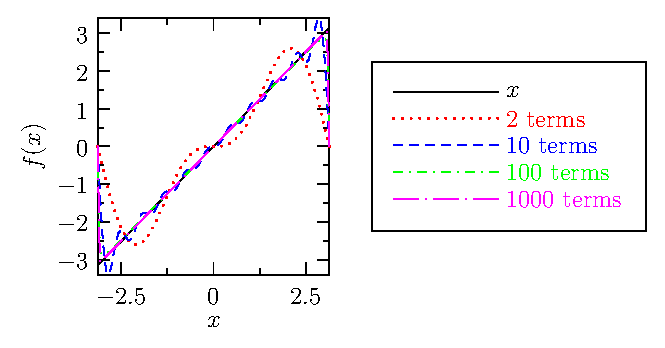
\includegraphics{201/fourierx}
    \caption{Fourier series approximations to $f(x)=x$.}
    \label{fourierx}
  \end{center}
\end{figure}
}

%FIXME: something about orthogonality? More examples?

\subsection{Problems}

\begin{enumerate}
  \item What are the Fourier sine and cosine series for
    $y=\sin x$?
    \hidesolution{
      Students should make use of the orthogonality property for $\sin nx$ and
      $\sin mx$, $n \neq m$.
    }
  \item What is the Fourier series for $f(x)$ if
    \be
    f(x) = \d(x-1)?
    \ee
  \item What is the Fourier series in $x$ for $f(x,t)$ if
    \be
    f(x,t) = 
    \left\{ \begin{array}{ll}
      -t           & \mbox{if $x < 0$};\\
      \phantom{-}t & \mbox{if $x \geq 0$}?
    \end{array} \right.
    \ee
    
  \item FIXME: add question on Gibbs phenomenom (NB: notes are written).
\end{enumerate}

\newpage
\section{Partial Differential Equations:
         \\Actually Solving Them}

Let us now return to the heat equation,
\be
\label{heateq}
\pp{y}{t} = \beta \frac{\partial^2y}{\partial x^2},
\ee
and add some \emph{initial conditions}
\be
y(x,0)=f(x)
\ee
and \emph{boundary conditions}
\be
\label{homdibc}
y(0,t)=0, \qquad y(\pi,t)=0.
\ee
Physically, this corresponds to modelling the temperature on a rod of length
$2\pi$ in contact at both endswith a heat sink with temperature $0$ (note
that this is not necessarily absolute zero: if we take $y=y+C$, the equation
remains the same, so our base temperature is arbitrary.) The
rod starts with the temperature at position $x$ given by $f(x)$.

We'll solve this using separation of variables:
\be
\label{heatF}
y = \sum_{n=0}^\infty T_n(t) X_n(x),
\ee
where we have taken $X_n(x)$ to be orthogonal\footnote{That is, if $n\neq m$, 
then $\int_0^\pi X_n(x) X_m(x) dx =0.$ This is the case with, elements of 
$\{\cos(nx),\sin(nx),n=0,1,\dots \}$.}.
Putting equation \eqref{heatF} into equation \eqref{heateq}, we get
\be
\label{heats}
\sum_{n=0}^\infty \ddt{T_n(t)}X_n(x)
=\beta\sum_{n=0}^\infty T_n(t)\ddtwo{X_n(x)}{x}
\ee
Now, since the $X_n$s are orthogonal, this actually holds term-by-term. That 
is, for each $n$, we have
\be
T_n'(t)X_n(x) = \beta  T_n(t)X_n''(x) 
\quad \implies \quad
\frac{1}{\beta}\frac{T_n'(t)}{T_n(t)}= \frac{X_n''(x)}{X_n(x)}.
\ee
Now, the LHS is independent of $x$, so the RHS must also be independent of $x$.
Since the RHS is also clearly independent of $t$, it must be constant. That is,
\be
\frac{1}{\beta}\frac{T_n'(t)}{T_n(t)}= \frac{X_n''(x)}{X_n(x)} = K_n,
\ee
where $K_n$ can only depend on $n$. 

This gives us an ODE for $X_n$,
\be
\label{Eigenfunction}
X_n'' = K_n X_n.
\ee
Now, depending on the sign of $K_n$, we have three possibilities, which we will
deal with by enforcing the boundary conditions. Since the $X_n$ are orthogonal,
the boundary conditions must be satisfied for each $n$. The cases are:
\begin{enumerate}
  \item $K_n=k_n^2 > 0$. In this case, $X_n(x)= C_1 e^{k_n x} +C_2 e^{-k_n x}$. 
    But then, $X_n(0)=0$ and $X_n(\pi)=0$ imply that $C_1=C_2=0$, so $X_n=0$ in 
    this case.
  \item $K_n = 0$. In this case, we get $X_n(x)=Ax +B$. Again, the boundary 
    conditions imply that $A=B=0$, so $X_n=0$ in this case.
  \item $K_n =-k_n^2 < 0$. This gives us periodic behaviour,
    \be
    X_n(x)=C_1\cos(k_nx) + C_2\sin(k_nx).
    \ee
    We require that $X_n(0)=C_1=0$, so we can remove all the cosines. The
    other boundary conditions gives us
    \be
    X_n(\pi)=C_2\sin(k_n\pi)=0,
    \ee
    which implies that either $C_2=0$ or $k_n$ is an integer. Since this is
    our last chance to have $X_n$ not be zero everywhere, we can't have $C_2=0$,
    so we set $k_n$ to be an integer. In particular, set $k_n=n$.
\end{enumerate}
Thus, $K_n=-n^2$, and $X_n= \sin(nx)$. Much simpler!

We now have enough information to start determining $T_n$. We know that 
$K_n=-n^2$, so $T_n$ obeys the equation
\be
T_n' = \beta K_n T_n = - \beta n^2 T_n 
\qquad \implies \qquad 
T_n = T_n(0) e^{-\beta n^2 t}.
\ee

Putting this together, our solution (so far) is
\be
y(x,t) = \sum_{n=0}^\infty T_n(0) e^{-\beta n^2 t} \sin(nx).
\ee
To get this, we have used the original equation and the boundary conditions. 
We still have to determine the values of $T_n(0)$, for which we will use the
initial conditions, $y(x,0)=f(x)$. That is,
\be
y(x,0)=f(x) =  \sum_{n=0}^\infty T_n(0) e^{-\beta n^2 t} \sin(nx)
= \sum_{n=0}^\infty T_n(0) \sin(nx).
\ee
In other words, this is just a sine-series for $f(x)$! However, instead of
integrating over $(-\pi,\pi)$, we only know $f(x)$ for $x\in(0,\pi)$. We can
solve this problem by extending $f(x)$ as an odd functions by setting 
$f(-x)=-f(x)$, so the coefficients are given by
\be
T_n(0)=\frac{1}{\pi}\int_{-\pi}^\pi f(x)\sin(nx)dx
=\frac{2}{\pi}\int_0^\pi f(x)\sin(nx)dx,
\ee
since the integrand is even.

The solution to the heat equation is then
\be
y(x,t)=\frac{2}{\pi}
\sum_{n=1}^\infty \[\int_0^\pi f(x)\sin(nx)\,dx\]
e^{-kn^2t}
\sin(nx), 
\ee

\workedexample{
  The initial temperature in a rod of length $\pi$ is given by
  \be
  \label{heat1ic}
  y(x,0)=2\sin(x)+\sin(5x),
  \ee
  and the temperature at the ends of the rod is kept at zero. Assuming that
  \be
  \pp{y}{t} = \beta \frac{\partial^2 y}{\partial x^2},
  \ee
  find $y(x,t)$ for $x\in(0,\pi)$, $t>0$.
  }{
  The boundary conditions match those given in equation \eqref{homdibc}, so
  the above analysis shows that we can express $y$ as a linear combination
  of $\{\sin(nx),n=1,2,\dots\}$. That is,
  \be
  y(x,t)=\sum_{n=1}^\infty T_n(0) e^{-\b n^2 t} \sin(nx).
  \ee
  The initial conditions are that $y(x,0)=2\sin(x)+\sin(5x)$, so $T_1(0)=2$,
  $T_5(0)=1$, and all others are zero. We can then write the solution as
  \be
  y(x,t) = 2 e^{-\b t} \sin(x) + e^{-25 \b t} \sin(5x).
  \ee
  This result is shown for various times in figure \ref{heat1} for $\b=1$.
  \begin{figure}[htbp]
    \begin{center}
      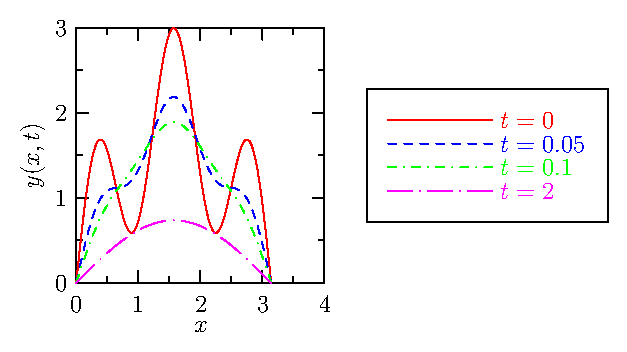
\includegraphics{201/heat1}
      \caption{The temperature at different times with initial conditions
        given in \eqref{heat1ic}.}
      \label{heat1}
    \end{center}
  \end{figure}
}


\subsection{Non-homogeneous constant boundary conditions}

Suppose that the boundary conditions were instead
\be
y(0,t)=A, \qquad y(\pi,t)=B.
\ee
Notice that these conditions match the the case $K_n=0$ with
\be
y(x,t)=\frac{B-A}{\pi}x+A.
\ee
This obeys the heat equation, since 
\be
\frac{\partial^2}{\partial x^2}(mx+b)=0= \pp{}{t}(mx+b),
\ee
and is independent of $t$, i.e.\ it is a steady state solution. Then, setting
\be
g(x) = f(x) - \(A+ \frac{B-A}{\pi}x\),
\ee
\be
\label{diribc}
y(x,t)=A + \frac{B-A}{\pi}x +
\frac{2}{\pi}
\sum_{n=1}^\infty\(\int_{0}^\pi g(x)\sin(nx)dx\) e^{-\b n^2t} \sin(nx)
\ee
matches both the initial and boundary conditions.

\workedexample{
  Solve the initial boundary problem
  \be
  \label{heat3ic}
  \pp{y}{t} = \b \pptwo{y}{x}, \qquad y(0)=1, \quad y(\pi)=1+\pi, 
  \quad y(x,0)=f(x)=x^2 +x +1
  \ee
  for $y(x,t)$.

}{
  The steady-state solution is $x+1$. Let
  \be
  g(x) = f(x) -(x+1) = x^2
  \ee
  Then,
  \be
  y(x,t) = 1 + x + \sum_{n=1}^\infty T_n(0) e^{-\b n^2 t} \sin(nx)
  \ee
  with
  \be
  x^2 = \sum_{n=1}^\infty T_n(0) \sin(nx).
  \ee
  The coefficients are given by the formula
  \be
  T_n(0) &=& \frac{2}{\pi} \int_0^\pi x^2 \sin(nx) \, dx
  \\\nonumber
  &=& \frac{2}{\pi}\[\left.x^2 \frac{-\cos(nx)}{n} \right|_0^\pi 
  + \frac{2}{n}\int_0^\pi x \cos(nx)dx\] 
  \\\nonumber
  &=& \frac{4}{n\pi}\[\left.\frac{s \sin(nx)}{n} \right|_0^\pi
  - \frac{1}{n}\int_0^\pi\sin(nx)dx  \] 
  \\\nonumber
  &=& \frac{4}{n^3\pi} \left.\cos(nx) \right|_0^\pi 
  = \frac{4(\(-1)^n-1\)}{n^3\pi}
  \ee
  The solution is therefore
  \be
  y(x,t) = 1+x+
  \sum_{n=1}^\infty \frac{4(\(-1)^n-1\)}{n^3\pi} e^{-\b n^2 t}\sin(nx).
  \ee
  as can be seen in figure \ref{heat3}.
  \begin{figure}[htbp]
    \begin{center}
      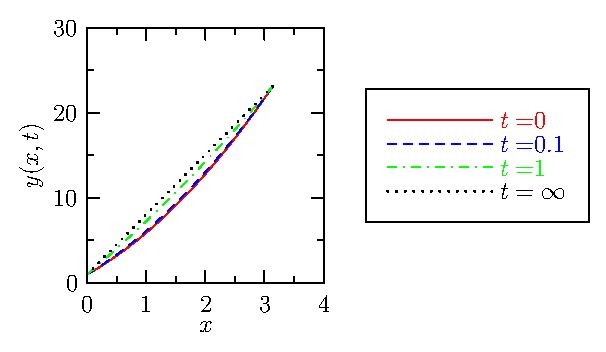
\includegraphics{201/heat3}
      \caption{The temperature at different times for the system given in 
        \eqref{heat3ic}.}
      \label{heat3}
    \end{center}
  \end{figure}

}

\subsection{A more complicated example}

\workedexample{
  The heat in a rod obey the equation
  \be
  \pp{y}{t}=\pptwo{y}{x}.
  \ee
  Given the boundary conditions 
  \be
  \label{heat2ic}
  y(0,t)=1 \qquad y(\pi,t)=e^\pi
  \ee
  and the and the initial condition $y(x,0)=e^x$, find $y(x,t)$.\\
}{
  The solution is given by
  \be
  y(x,t)&=&1 + \frac{e^\pi-1}{\pi}x +
  \sum_{n=1}^\infty T_n(0) e^{-n^2t} \sin(nx),
  \\ 
  T_n(0)&=&\frac{2}{\pi}\int_{0}^\pi g(x)\sin(nx)dx,
  \\ 
  g(x)&=&e^x - 1 - \frac{e^\pi-1}{\pi}x.
  \ee
  From equation \eqref{Fourierx}, we have
  \be
  x = 2 \sum_{n=1}^\infty  \frac{(-1)^{n+1}}{n} \sin(nx)
  \ee
  To find the Fourier sine-series for $e^x$, we must compute
  \be
  a_n = \frac{2}{\pi}\int_0^\pi e^x \sin(nx) \, dx 
  = \frac{2}{\pi}\left.\frac{e^x\(\sin(nu) - n \cos(nu)\)}{n^2+1}\right|_0^\pi
  = \frac{2}{\pi}\frac{n(1 - (-1)^ne^\pi)}{n^2+1}
  \ee
  Also, the Fourier series for $1$ over $x\in(-\pi,\pi)$ has coefficients
  \be
  \frac{2}{\pi}\int_0^\pi \sin(nx) = \frac{2}{n\pi}\left.\cos(nx) \right|_0^\pi
  = \frac{2\((-1^n)-1\)}{n\pi},
  \ee
  so, over $x\in(0,\pi)$,
  \be
  1 = \sum_{n=1}^\infty \frac{2\((-1^n)-1\)}{n\pi} \sin(nx).
  \ee
  
  Noting that the Fourier series is a linear, so we can add the series together:
  \be
  e^x - 1- \frac{e^\pi}{\pi}x
  &=& \sum_{n=1}^\infty \frac{2}{\pi}n\frac{1 - (-1)^ne^\pi}{n^2+1} \sin(nx)
  - \frac{e^\pi-1}{\pi} 2 \sum_{n=1}^\infty  \frac{(-1)^{n+1}}{n} \sin(nx)
  \\ \nonumber
  &&-\sum_{n=1}^\infty \frac{2\((-1^n)-1\)}{n\pi} \sin(nx)
  \\ \nonumber
  &=&\sum_{n=1}^\infty \(\frac{2}{\pi}\frac{n(1 - (-1)^ne^\pi)}{n^2+1} 
  -\frac{e^\pi-1}{\pi}2 \frac{(-1)^{n+1}}{n}- \frac{2\((-1^n)-1\)}{n\pi}\)
  \sin(nx).
  \ee
  Now, this is all a bit messy, but we do end up with the solution
  \be
  y(x,t) = 1 &+& \frac{e^\pi-1}{\pi}x
  \\ \nonumber
  &+& 
  \sum_{n=1}^\infty \(\frac{2}{\pi}\frac{n(1 - (-1)^ne^\pi)}{n^2+1} 
  -2 \frac{e^\pi-1}{\pi} \frac{(-1)^{n+1}}{n}- \frac{2\((-1^n)-1\)}{n\pi}\)
    e^{-n^2t} \sin(nx),
  \ee
  as can be seen in figure \ref{heat2}.
  \begin{figure}[htbp]
    \begin{center}
      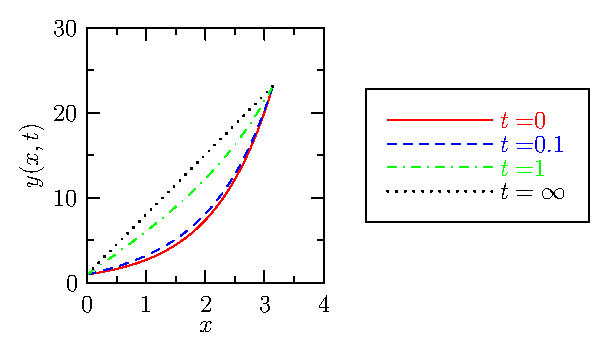
\includegraphics{201/heat2}
      \caption{The temperature at different times with initial conditions
        given in \eqref{heat2ic}.}
      \label{heat2}
    \end{center}
  \end{figure}
}



\subsection{Problems}

\begin{enumerate}
  \item 
    Show that equation \eqref{diribc} does indeed solve the heat equation
    with the given boundary and initial conditions.
  \item 
    An inanimate carbon rod of length $\pi$ is hit with a ``laser'', 
    transferring an amount of heat $H$ to a point at its centre. That is, the
    initial temperature distribution along its length is given by
    \be
    y(x,0)=H\delta\(x-\frac{\pi}{2}\).
    \ee
    If the ends of the rod are kept at constant temperature $0$, and the 
    temperature in the rod obeys the relationship
    \be
    \pp{y}{t} = \beta \frac{\partial^2 y}{\partial x^2},
    \ee
    find $y(x,t)$ for all $t\geq 0$.
    \hidesolution{
      Following the above procedure,
      \bee
      y(x,t)=\frac{2}{\pi}
      \sum_{n=1}^\infty T_n(0) e^{-kn^2t} \sin(nx)
      \eee
      with 
      \bee
      T_n(0) &=& \frac{2}{\pi}\int_0^\pi H \d\(x-\frac{\pi}{2} \) \sin(nx) \, dx
      \\
      &=& \frac{2H}{\pi} \sin\(\frac{n\pi}{2}\)
      \\
      &=& \frac{2H}{\pi}
      \left\{ \begin{array}{ll}
        0,           & \mbox{if $n=2m$}\\
        \sin\(m\pi+ \frac{\pi}{2}\), & \mbox{if $n=2m+1$}
      \end{array} \right.
      \\
      &=& \frac{2H}{\pi}
      \left\{ \begin{array}{ll}
        0,           & \mbox{if $n=2m$}\\
        (-1)^m, & \mbox{if $n=2m+1$}.
      \end{array} \right.
      \eee
      The solution is then given by
      \bee
      y(x,t) = \frac{2H}{\pi} \sum_{m=0}^\infty (-1)^m e^{-4\beta m^2 t} \sin(2mx)
      \eee
    }
  \item
    \emph{Neumann boundary conditions} specify the value of the function at
    the boundary, e.g. $y(0,t)=A$, $y(\pi,t)=B$ with $A$ and $B$ constant.
    We showed that the set of Eigenfunctions given by equation 
    \eqref{Eigenfunction} must be $\{\sin(nx),n=1,2,\dots\}$ in this case. 
    If the boundary conditions were instead \emph{Dirichlet boundary conditions}
    such as
    \be
    \left.\pp{y(x,t)}{x}\right|_{x=0}=0, \qquad
        \left.\pp{y(x,t)}{x}\right|_{x=\pi}=0,
    \ee
    what are the Eigenfunctions?


\end{enumerate}

%\newpage
%\section{Last section thing}
%FIXME: add some interal tables, trig identities, and whatnot.

\end{document}
